\documentclass[useAMS,usenatbib]{mnras}
\usepackage[]{natbib,amsmath,amssymb,times,refname,bm}
\bibpunct{(}{)}{;}{a}{}{,}
%\linespread{1.0}
%\usepackage[utf8]{inputenc}
\usepackage{tabularx,amsmath,amssymb,hyperref}
\usepackage{graphicx,epsfig,color,latexsym}

\renewcommand{\d}{\mathrm{d}}
\newcommand{\e}{\mathrm{e}}
\newcommand{\ii}{\mathrm{i}}
\newcommand{\bea}{\begin{eqnarray}}
\newcommand{\eea}{\end{eqnarray}}
\newcommand{\be}{\begin{equation}}
\newcommand{\ee}{\end{equation}}
\newcommand{\rund}[1]{\left(#1\right)}
\newcommand{\vc}[1]{\mbox{\boldmath $#1$}}
\newcommand{\dc}{\partial}
\newcommand{\eck}[1]{\left[ #1 \right]}

\newcommand{\msun}{\,h^{-1}\,M_{\odot}}
\newcommand{\iobs}{I^{\rm obs}}
\defcitealias{Semboloni13}{S13}

\long\def\/*#1*/ {}

%\def\llabel#1{\label{sc:#1}  {#1}\hspace{0.5cm}}
%\def\elabel#1{\label{eq:#1}\fbox{#1}}
\def\llabel#1{\label{sc:#1}}
\def\elabel#1{\label{eq:#1}}

\sloppy

\title[Colour gradient bias]
{Calibration of colour gradient bias in shear measurement using CANDELS}
\author[Xer et al.]%
{
X. Er$^1$ \thanks{er.xinzhong@oa-roma.inaf.it},
H. Hoekstra$^2$, T. Schrabback$^3$, V. F. Cardone$^1$, R. Scaramella$^1$, R. Maoli$^4$,
\newauthor{M. Vicinanza$^{1,4,5}$, B. Gillis$^{6}$ L. Miller$^{7}$, J. Rhodes$^{8,9}$}
\\
$^1$ I.N.A.F. - Osservatorio Astronomico di Roma, via Frascati 33, 00040 - Monte Porzio Catone, Roma, Italy\\
$^2$Leiden Observatory, Leiden University, PO Box 9513, NL-230 RA, Leiden, the Netherlands \\
$^3$Argelander Instutite fuer Astronomie, Auf dem Huegel 71, D-53121 Bonn, Germany\\
$^4$Dipartimento di Fisica, Universita di Roma "La Sapienza", Piazzale Aldo Moro, 00185 - Roma, Italy\\
$^5$Dipartimento di Fisica, Universita di Roma "Tor Vergata", via della Ricerca Scientifica 1, 00133 - Roma, Italy\\
$^6$Royal Observatory, University of Edinburgh, Blackford Hill, Edinburgh EH9 3HJ, UK\\
$^7$Department of Physics, Oxford University, keble Road, Oxford OX I 3RH, UK\\
$^8$Jet Propulsion Laboratory, California Institute of Technology, 4800 Oak Grove Drive, Pasadena, CA 91109, USA\\
$^8$California Institute of Technology, 1200 East California Blvd, Pasadena, CA 91125, USA
%$$
}
\date{Accepted --;  received --;  in original from \today}
\pubyear{2016}

\begin{document}
\maketitle

\begin{abstract}
{\it Euclid} will image about two billion galaxies that can be used to infer cosmological
parameters using weak gravitational lensing. Exploiting the precision afforded by these
data relies critically on our ability to correct for instrumental effects, such as the convolution
by the point spread function (PSF). A complication is the fact  that the optical data
are obtained using a broad bandpass (550-920\,nm) while the diffraction-limited PSF depends
on wavelength. This leads to biases in the recovered galaxy shapes because the colours of 
galaxies vary spatially. 
We show that the colour-gradient bias can be determined with high accuracy in simulated
noisy data. We also find that higher order image distortions, such as flexion, enhance
the bias, which may be relevant for the study of lensing in high density regions.
We estimate the size of this colour-gradient biases using multi-band observations 
from the {\it Hubble} Space Telescope and find correlations with the colours and sizes of
the galaxies, but do not observe a significant dependence with redshift. 
{\bf We need some concluding remark about the impact for Euclid.}

\end{abstract}
\begin{keywords} cosmology, weak lensing, systematics
\end{keywords}

%\vspace{1.0\baselineskip}

\section{Introduction}

The images of distant galaxies are distorted, or sheared, by the tidal effect of the gravitational  potential generated by intervening matter, an effect commonly referred to as weak gravitational lensing
\citep[e.g.][for a detailed introduction]{Bartelmann01}. The measurement of the resulting correlations in the shapes can be used to directly infer the statistical properties of the mass distribution in the Universe, which in turn provide constraints on cosmological parameters.
Hence weak gravitational lensing by large-scale structure, or cosmic shear, has been identified as a powerful tool for cosmology. The measurement of the signal as a function of cosmological time 
is sensitive to the expansion history and the growth rate of large-scale structures, and can be used to constrain models for dark energy and modified gravity.

A useful measurement of the cosmic shear signal requires averaging over large numbers of galaxies
to reduce the uncertainty caused by the intrinsic ellipticities of galaxies. The result is, however, only meaningful if biases in the shape estimates are negligible. Various instrumental effects change the observed ellipticities by more than the typical lensing signal, which is of order one per cent.
The most dominant source of bias is the smearing of the images by the point spread function (PSF),
driving the desire for space-based observations \citep{Paulin-Henriksson08, Massey13}.
Despite these observational challenges, the most recent cosmic shear studies are starting to yield competitive constraints on cosmological parameters \citep{Heymans13, Jarvis16,Jee16,Hildebrandt17}.
These results are based on surveys of modest areas of the sky, which limits their ability to study the nature of dark energy, which requires more than an order of magnitude improvement in precision.

Such a measurement is the objective of {\it Euclid} \citep{Laureijs11}, the dark energy mission of the European Space Agency (ESA) scheduled for a launch in 2020, which will survey the 
15\,000 deg$^2$ of extragalactic sky that has both low extinction and zodiacal light. To reduce the detrimental effects of noise on the shape measurements, the images used for the lensing analysis are observed using a wide bandpass (550-920\,nm). The much smaller PSF in space-based observations 
is a major advantage, but the diffraction-limited PSF leads to new complications. 

The most prominent one is that the correction for the smearing by the chromatic PSF depends on the spectral energy distribution (SED) of the galaxy of interest \citep{Cypriano10, Eriksen17} and gnoring this would lead to significant biases in the case of {\it Euclid}. Fortunately this can be accounted for using the supporting broad-band observations that are used to derive photometric redshifts for the sources: the correction employs an effective PSF which is derived from the estimate of the observed SED of the galaxy. This correction is sufficient if the SED does not vary spatially \citep{Eriksen17}. If this is not the case, the underlying brightness distribution, which is needed for an unbiased estimate of the shear, cannot be unambiguously recovered from the observed images.
This results in a higher order systematic bias, which we call colour-gradient (hereafter CG) bias.
As shown by \cite{Semboloni13} (S13 in the rest of this paper) the amplitude depends on several factors: the SED of the galaxy, the relative size of the galaxy to the PSF, and the width of the bandpass, $\Delta\lambda$.  For instance, the bias scales as $\Delta\lambda^2$, and thus is particularly relevant in the case of {\it Euclid}.

Galaxies show a wide variety in colour gradients, with elliptical galaxies typically showing negative colour gradients (redder in the centre and bluer in the outskirts), with steeper gradients more commonly found in bluer or more luminous early type galaxies \citep[e.g.][]{2011MNRAS.414.3052D,
2011MNRAS.411.1151G}. \citet[][]{2010AJ....140.1528L, 2016A&A...593A..84K} also suggest
correlations between colour gradients and the overall colours and luminosities of the galaxies.
Hence the relation between galaxy morphology and density may cause the CG bias to vary across the sky and lead to correlations with the lensing signal itself. 

It is important that all systematic sources of biases are accounted for to a level that is smaller than the 
statistical uncertainties. In the case of {\it Euclid} this leads to tight requirements, as detailed in 
\citep[e.g.][]{Massey13,Cropper13}. Initial studies by \cite{Voigt12} and \citetalias{Semboloni13} used simulated images to show that the CG bias could be substantial,
exceeding nominal requirements for the multiplicative bias in the shear. They also argued
that it should be possible to calibrate the bias using {\it Hubble} Space Telescope (HST) observations
of a large sample of galaxies in the F606W and F814W filters. However, their conclusion is based on the analysis of simulated noiseless data. In this work, we revisit the issue of the calibration of CG bias,
with a particular focus on determining the bias from data with realistic noise levels. 

In Section~\ref{sec:concepts}, we describe the main concepts and introduce the notation. We present the results from the analysis of simulated images in Section~\ref{sec:simulations}. In particular we explore the  impact of having to use noisy data to measure the CG bias in Section~\ref{sec:noisy}.
In Section~\ref{sec:candels} we estimate the CG bias using HST observations from the Cosmic Assembly Near-infrared Deep Extragalactic Legacy Survey \citep[CANDELS;][]{candelsref}.

%%%%%
\section{The origin of colour gradient bias}
\label{sec:concepts}

Following the notation of \citetalias{Semboloni13}, we consider an image of a galaxy, and denote the photon brightness
distribution of the image at each position $\bm \theta$ and wavelength $\lambda$ by $I({\bm \theta};\lambda)$, which is related to the intensity $S({\bm\theta};\lambda)$ by $I^0(\theta;\lambda)=\lambda S({\bm\theta};\lambda)
T(\lambda)$, where $T(\lambda)$ is the normalised transmission. We take this to be a top-hat with a
width $\Delta\lambda$ around a central wavelength $\lambda_{\rm cen}$. The resulting image of the galaxy, observed using a telescope with a PSF $P({\bm \theta};\lambda)$  is given by:
%
\be
I^{\rm obs}({\bm\theta}) = \int_{\Delta\lambda} I^0({\bm\theta}; \lambda) *  
P({\bm \theta},\lambda)\, \d \lambda,
\label{eq:iobs}
\ee
%
where $*$ denotes a convolution. 

A measurement of the ellipticity of a galaxy provides an unbiased (but noisy) estimate of the 
weak gravitational lensing signal, quantified by the complex shear $\gamma=\gamma_1+\ii\gamma_2$.
The ellipticity $\epsilon$ in turn can be determined from the second order brightness moments $Q^0_{ij}$ of the PSF-corrected image $I^0(\theta)$ \citep{2001PhR...340..291B}:
%
\be
\epsilon_1+\ii \epsilon_2 \approx \frac{Q^0_{11} - Q^0_{22} + 2 \ii Q^0_{12} }
{Q^0_{11} + Q^0_{22} +2(Q^0_{11}Q^0_{22} - (Q^0_{12})^2)^{1/2}}
\elabel{mshear}
\ee
%
where the second order brightness moments are given by\footnote{We implicitly assume that the moments are evaluated around the position where the dipole moments vanish.}
%
\be
Q^0_{ij} = {1 \over F} \int  I^{0}({\bm \theta})\, \theta_i \theta_j \, \d^2 {\bm \theta} \quad\; (i,j=1,2),
\ee
%
where $F=\int \d^2{{\bm\theta}}  I^{0}({\bm\theta})$ is the total observed photon flux.

In practice, however, the observed moments are measured from the PSF-convolved image given by
Eqn.~(\ref{eq:iobs}). Moreover, the moments are evaluated using a weight function $W({\bm\theta})$  to reduce the effect of noise in the images. Hence, the observed quadrupole moments are given by
\be
Q^{\rm obs}_{ij} = {1 \over F_{\rm w}} \int_{\Delta\lambda} \d\lambda \int \d^2 {\bm\theta} \,
I^0(\theta; \lambda) *  P(\theta,\lambda)\, \theta_i \theta_j \, W({\bm \theta})\,,
\ee
%
where $F_{\rm w}$ is the weighted flux. The use of a weight function biases the observed moments, 
and the aim of moment-based shape measurement algorithms is to correct for this using estimates of the higher order moment \citep[e.g.][]{Kaiser1995,Melchior11}. An alternative approach is to fit sheared, PSF-convolved models to the observed images 
\citep[e.g.][]{Bridle02,Miller13}; in these fitting methods the profile itself acts as a weight. 

\citetalias{Semboloni13} showed that the inevitable use of a weight function gives rise to the CG bias, which
scales as $\Delta\lambda^2$. The bias also depends on the choice of the weight function,
and vanishes in the case of {\it unweighted} moments. In the latter case it possible to determine the PSF-corrected moments $Q^0_{ij}$ from the observed quadrupole moments because
%
\be
Q^{\rm obs}_{ij}=Q^0_{ij}+P^{\rm eff}_{ij} \,
\ee
%
where $P^{\rm eff}_{ij}$ are the quadrupole moments of the effective PSF,  defined as
\be
P_{\rm eff}({\bm \theta}) = \frac{1}{F} \int \d \lambda\, P({\bm \theta},\lambda)\, F(\lambda) \,,
\ee
where   $F(\lambda)$ is the photon flux as a function of wavelength, which is directly related to the spectral energy distribution (SED) of the galaxy. Hence the correction for the chromatic PSF requires an estimate of the SED.  \cite{Eriksen17} have shown that the broadband observations that are used to determine photometric redshifts for {\it Euclid} can also be used to estimate the effective PSF with sufficient accuracy to meet the stringent requirements presented in \cite{Cropper13}.

%
\begin{figure*}
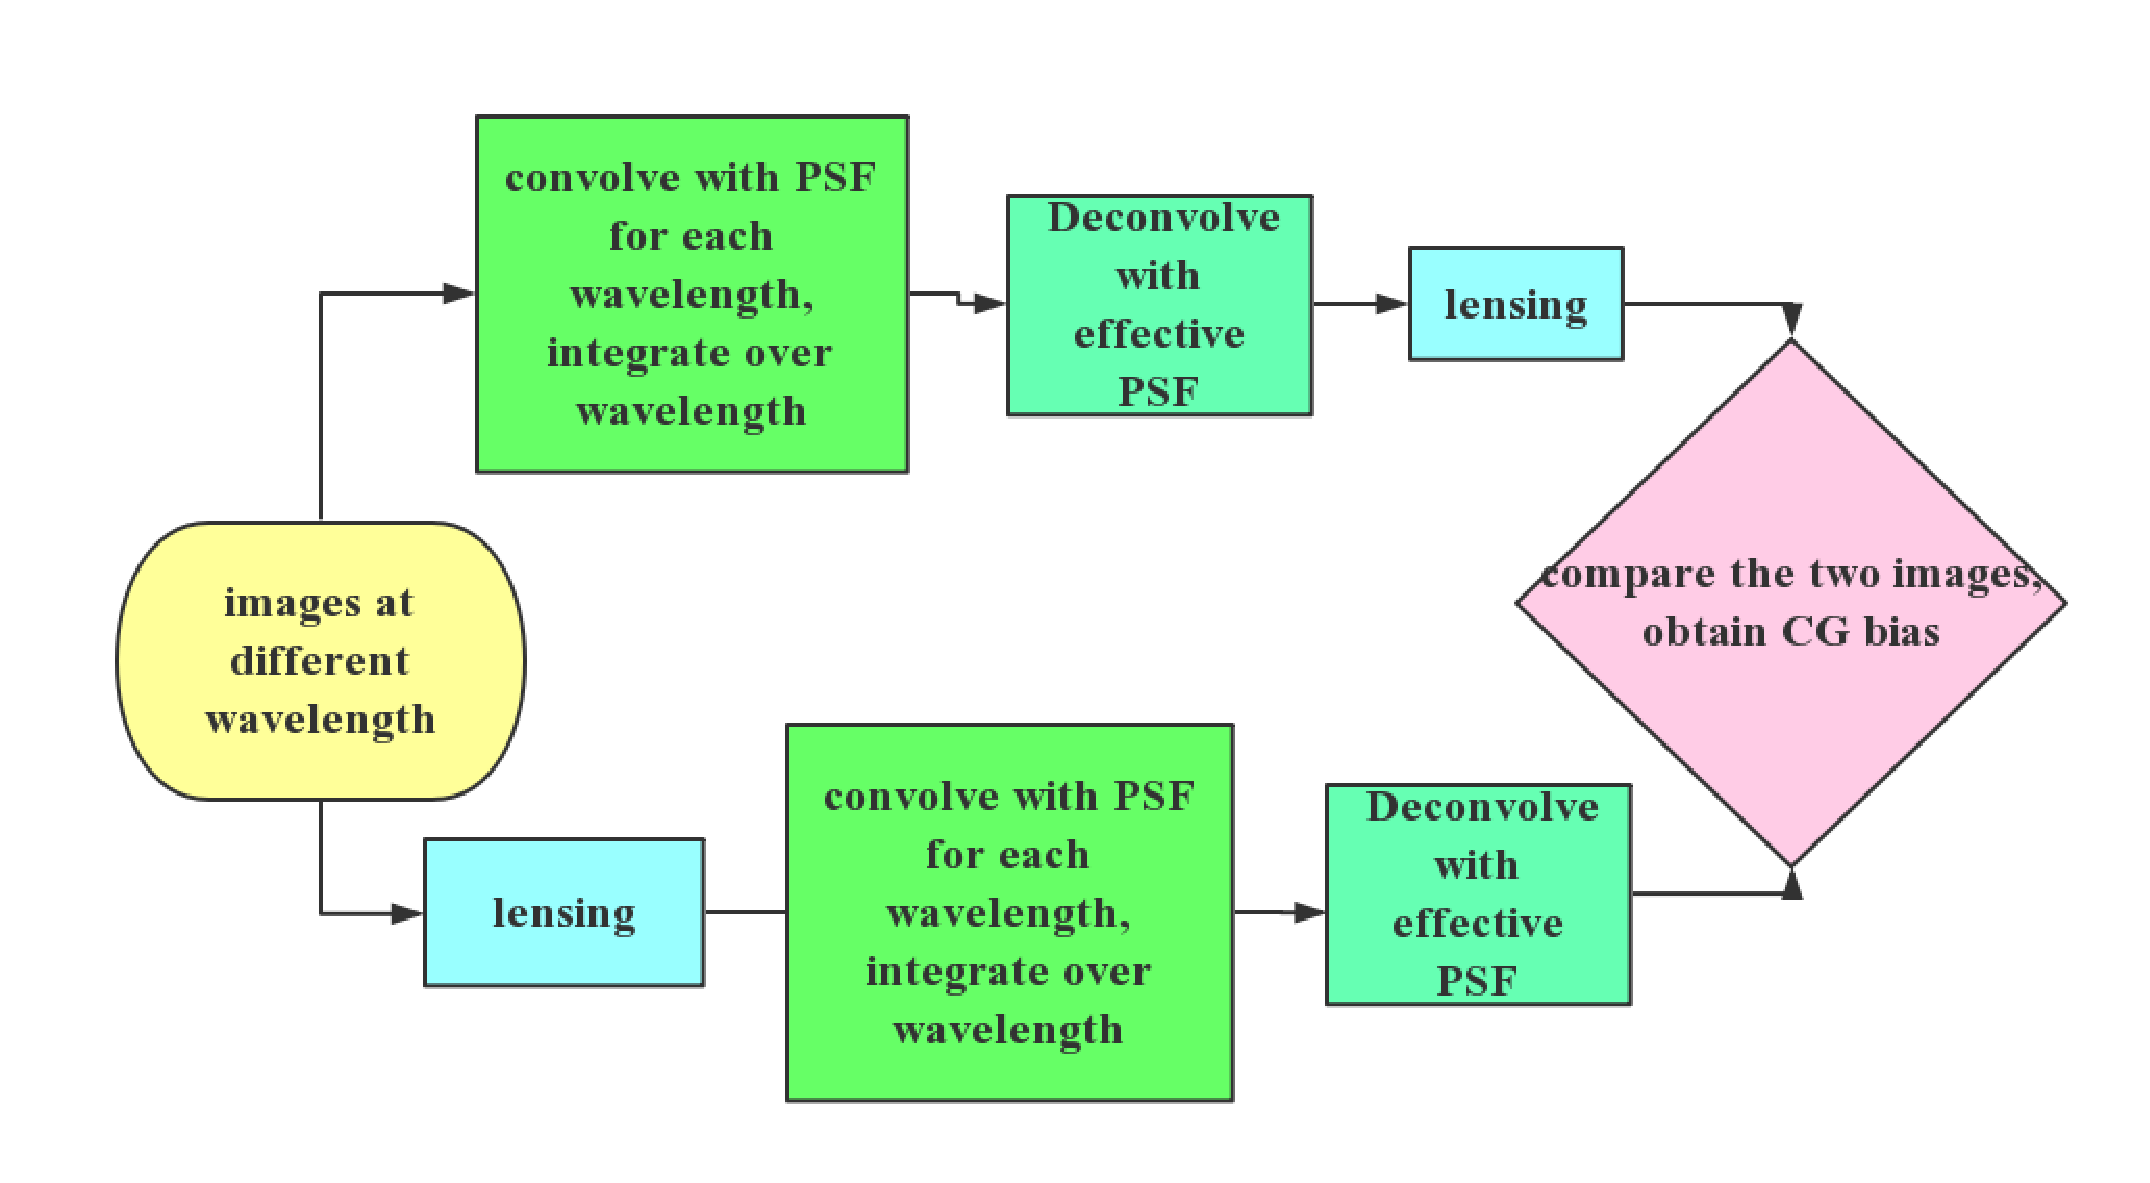
\includegraphics[width=12.5cm]{colourg.eps}
\caption{Flowchart describing how the colour-gradient bias is determined. The initial image
is the same in both flows, but in the top flow an image without a colour gradient is created
to which a shear is applied. In the bottom flow, the image is sheared before the PSF steps
are applied. The ellipticities of the resulting images differ slightly, and can be used to quantify
the bias that is introduced.}
\label{fig:flowchart}
\end{figure*}
%

Our approach to evaluate the multiplicative bias in the lensing signal that is introduced by colour gradient is similar to the one in \citetalias{Semboloni13}. Figure~\ref{fig:flowchart} shows the flowchart of the steps that enable us to evaluate the CG bias.  In both cases we start with the same wavelength dependent image $I^0({\bm \theta};\lambda)$, but the bottom flow resembles what happens in the actual observations: the original image is sheared\footnote{We use 
$\gamma_1=0.05$  and $\gamma_2=0.02$ as reference, but we verified that other values yield simialr results.} before the convolution with the PSF. The deconvolution with the effective PSF then yields the PSF-corrected shape. In the top flow the PSF steps are applied first, resulting in an image without a colour gradient that is subsequently sheared.

We measure the ellipticities of the resulting images to estimate the CG bias. To reduce noise in our estimate of the multiplicative bias $m$ we use the ring-test method \citep{Nakajima07} where we create eight copies of the original galaxy but with different orientations. The ensemble averaged ellipticities then  provide an estimate of the multiplicative CG bias, $m$ (we do not explore additive bias here), via
%
\be
m= {\epsilon_i^{\rm CG} \over \epsilon_i^{\rm NCG} }-1,
\ee
%
where `CG' indicates the case where the galaxy has a colour gradient, and `NCG' is the galaxy
with a uniform colour. Note that our approach differs slightly from that in \citetalias{Semboloni13}, who quantify the
response of the observed ellipticity to an applied shear. Hence, they do not apply the last step
in the bottom flow (the deconvolution), but rather convolve the final image in the top flow. 
The steps presented in Fig.~\ref{fig:flowchart} yield a more symmetric result, highlighting the fact
that the CG bias is the consequence of the fact that the shearing of the image does not commute with the convolution with the PSF. However, we verify in Sect.~\ref{sec:simulations} that we recover
the results of \citetalias{Semboloni13} (see Fig.~\ref{fig:biasofweight}).

\section{Colour gradient bias in simulated data}
\label{sec:simulations}

The CG bias is a higher order systematic bias, and thus the changes in the measured
ellipticities are small. It is therefore important to verify that numerical errors in the calculations
are subdominant compared to the small effects we aim to measure. To do so, we compare
results from two independent codes that are used to generate the simulated images: one is
written in C/C++ and the other uses the python-based {\tt GalSim} package
\citep{2015A&amp;C....10..121R}, which is widely used to created simulated images
\citep[e.g.][]{FenechConti17, Hoekstra16}. {\bf Er: please check if this is correct.} In the C code we compute the image by multiplying the  surface brightness at the centre of each pixel using a sheared S{\'e}rsic profile with the pixel area. In the case of {\tt GalSim} we use the {\tt Shear()} function
(which convolves the image by the pixel). Since we are interested in small differences in the shapes of deconvolved images, we checked for numerical errors. We convolved and subsequently deconvolved elliptical images. Comparison of the recovered ellipticities revealed small differences
between the codes that ranged from  $10^{-7}$ to $10^{-6}$, two orders of magnitude smaller
than the CG biases we are concerned with. Hence can safely neglect this numerical artefacts here.

As a further test we compare directly to the results obtained by \citetalias{Semboloni13} for two reference galaxy models. 
The reference galaxies are modeled as the sum of a bulge and disk component. To describe the wavelength dependence of the images we use the galaxy SED templates from \citet{1980ApJS...43..393C}: we use the SED for an elliptical galaxy for the bulge and take the SED of an irregular galaxy for the disk. This choice ensures that the resulting colour gradients are large. The two components are 
described by a circular S{\'e}rsic profile:
\be
I_{\rm S}(\theta) = I_0 {\rm e}^{-\kappa\; \left(\frac{\theta}{a}\right)^{1/n}},
\ee
%
where $I_0$ is the central intensity, and $\kappa=1.9992\,n -0.3271$. For the bulge component we adopt $n=1.5$ and for the disk we use $n=1$. The profiles are normalised such that the bulge contains 25\% of the flux at a wavelength of 550\,nm. The galaxies are circular and the sizes for the bulge and disk for galaxy `B'   are $0\farcs17$ and $1\farcs2$, respectively. The second galaxy `S' is smaller with sizes of $0\farcs09$ and $0\farcs6$  for the bulge and disk, respectively (also see Table~3 in \citetalias{Semboloni13}).
We create images with a size of  $256\times256$ pixels, and resolution $0.05$ arcsec/pixel at 
wavelengths 1\,nm apart and sum these in the range $[550:\,920]$\,nm to mimic the {\it Euclid} pass-band.

To create the PSF-convolved images we consider several PSF profiles. For a direct comparison with \citetalias{Semboloni13} use their reference PSF (PSF1), which is a Gaussian with a wavelength dependent dispersion
%
\be
\sigma_{\rm PSF}(\lambda) = 0\farcs102\rund{\lambda \over 800{\rm nm}},
\elabel{psf}
\ee
%
As discussed in \citetalias{Semboloni13} this PSF has a similar size as the nominal {\it Euclid} PSF, but a steeper wavelength-dependence. To approximate the {\it Euclid} PSF they consider a model that 
consists of a compact Gaussian core and an appropriately scaled top-hat (PSF3 in \citetalias{Semboloni13}).
Instead we use here a more realistic obscured Airy profile, which is actually close to the {\it Euclid}
design profile \citep{Laureijs11}:
%
\be
P(\theta) = {I_0 \over (1-\epsilon^2)^2} \rund{{2J_1(x)\over x} - {2\epsilon J_1(\epsilon x) \over x}}^2,
\elabel{psfairy}
\ee
%
where $I_0$ is the maximum intensity at the center, $\epsilon$ is the aperture obscuration ratio, and $J_1(x)$ is the first kind of Bessel function of order one; $x$ is defined as $x=\pi \theta/\lambda\, D $.
In the case of {\it Euclid} $D=1.2$m and $\epsilon=1/3$. We compare this model to the Gaussian
case and PSF3 from \citetalias{Semboloni13} in Fig.~\ref{fig:psfmodel} at the 550\,nm and 920\,nm.

\begin{figure}
\centerline{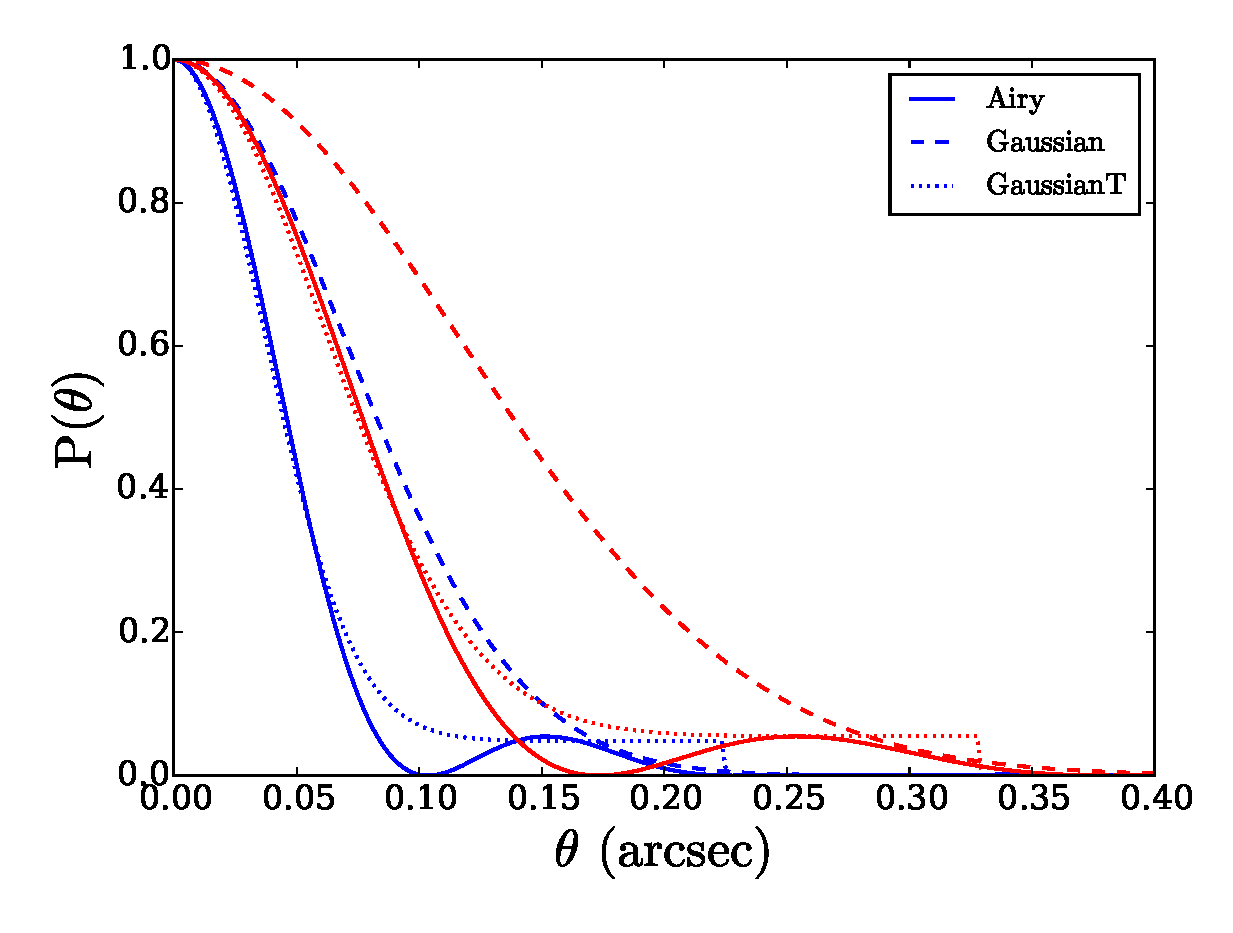
\includegraphics[width=\hsize]{zairy.eps}}
\caption{Comparison of the obscured Airy profile (solid), which is a good approximation
to the {\it Euclid} PSF, to PSF1 (Gaussian; dashed) and PSF3 (compact Gaussian and 
top-hat; dotted) from \citetalias{Semboloni13}. The profiles for 550\,nm are indicated by the blue lines and
the results for 920\,nm are shown in red.}
\label{fig:psfmodel}
\end{figure}
%


% HH: I think the table is not really necessary here as we are not comparing biases for the 
% different PSFs as was done in \citetalias{Semboloni13}
%
%\begin{table}
 % \begin{tabular}{|l|l|}
%    \hline\hline
%    PSF  &Description\\
%    \hline
%    Gaussian &Gaussian PSF described by Eq.\,\ref{eq:psf} with $w_{0,800}=0.102$\\
%    \hline
%    GaussianT &Gaussian core described by Eq.\,\ref{eq:psf} with $w_{0,800}=0.054$\\
%    &plusing top-hat with 20 percent of the total flux\\
%    &the cut-off size $\propto\lambda^{0.74} (\citetalias{Semboloni13})$\\
%    \hline
%    Airy  &Airy model with obscuration $1/3$ (Eq.\ref{eq:psfairy})\\
%    \hline
%  \end{tabular}
%  \caption{\label{table:psfmodel}The PSF models shown in
%    Fig.\,\ref{fig:psfmodel}.  The Gaussian model, which is the same
%    PSF model in \citetalias{Semboloni13} is used for the simulated images.  The GaussianT
%    model is a Gaussian core plus a top hat function (\citetalias{Semboloni13}), which is
%    shown as a comparison with Airy model.  The Airy model is used for
%    the bias calibration and HST data analysis in the following
%    section.}
%\end{table}
%

As a test of our implementation of the pipeline to determine the CG bias we compare our results to those from \citetalias{Semboloni13}. We reproduced all their results, but here we only show the comparison when 
$\theta_{\rm w}$, the width of the weight function that is used to compute the quadrupole moments, is varied. As discussed in Sect.~\ref{sec:concepts} the amplitude of the noise bias depends on the width of the weight function that is used to compute the (weighted) quadrupole moments. 

The results of this test are presented in Fig.~\ref{fig:biasofweight}. The solid lines indicate the results from \citetalias{Semboloni13} for the two reference galaxies B (red) and S (blue). We compare these to the outcome of the C code (dashed lines) and the {\tt GalSim} code (dotted lines). The agreement is excellent for the large galaxy (B) for the full range in $\theta_{\rm w}$. Our two codes agree also well for the small galaxy (S), but the difference with \citetalias{Semboloni13} is noticeable. However, given the consistent results between the C and {\tt GalSim} code we conclude that numerical errors are negligible in our implementation. In the remainder, we limit the simulations to those generated with {\tt GalSim}.

{\bf Do we understand why there is a difference for the blue lines? I see there is a comment in the 
tex file that the parameters for the galaxies were slightly different? Can this be fixed?}
%(the reason for the small divergence of blue lines is that the
%parameters used for simulating galaxy are slightly different).

Figure~\ref{fig:biasofweight} shows that the CG bias decreases rapidly when the width of the weight function is increased. This allows for an interesting trade-off between CG bias and noise bias. The latter increases with increasing $\theta_{\rm w}$ but relatively slowly (see Fig.~4 in \citetalias{Semboloni13}). As a proxy for the optimal weight function (which maximizes the signal-to-noise ratio) we adopt the value of the 
half-light radius in the remainder of this paper. This yield $m=0.8\times10^{-3}$ for galaxy B and
$m=2\times10^{-3}$ for galaxy S, demonstrating that the CG bias is a strong function of galaxy size.


\subsection{Impact for large distortions}

{\bf Er: please add text to explain what you did and add the figure with the flexion
results.} Besides shear, there are higher order image distortions in weak lensing,
such as flexion \citep[e.g.][]{2002ApJ...564...65G,bacon2006}. In
previous analysis, we only consider the shear effect in the lensing
process, while the higher order image distortions also suffer from CG
bias as well. In additional tests, we perform the complete lens
ray-tracing instead of solely shearing the images. (We only use our C
code in this part, since the current version of GalSim only provides
shear effect.) We adopt an Singular Isothermal Sphere halo model as
the lens model, and vary the configuration within some reasonable
range, such as the Einstein radius, and the separation between the
lens and the source image (the corresponding shear value varies
between about $[0.02, 0.1]$). We find that the variation of lensing
magnitude can cause different CG bias (yellow shadow in
Fig.\ref{fig:biasofweight}), and in most time the flexion effect will
increase the CG bias. Such effects do not appear if we solely shear
the images. However in general case, the cosmic shear has a value
about a few percents. We can see that from the bottom boundary of the
yellow shadow, the bias are almost the same as that only considering
the shear effect. Only in case of the galaxy cluster lensing,
galaxy-galaxy lensing, especially in the strong lensing region, when
the flexion becomes significant, one has to take into account of such
kind of effect.


%
\begin{figure}
\centerline{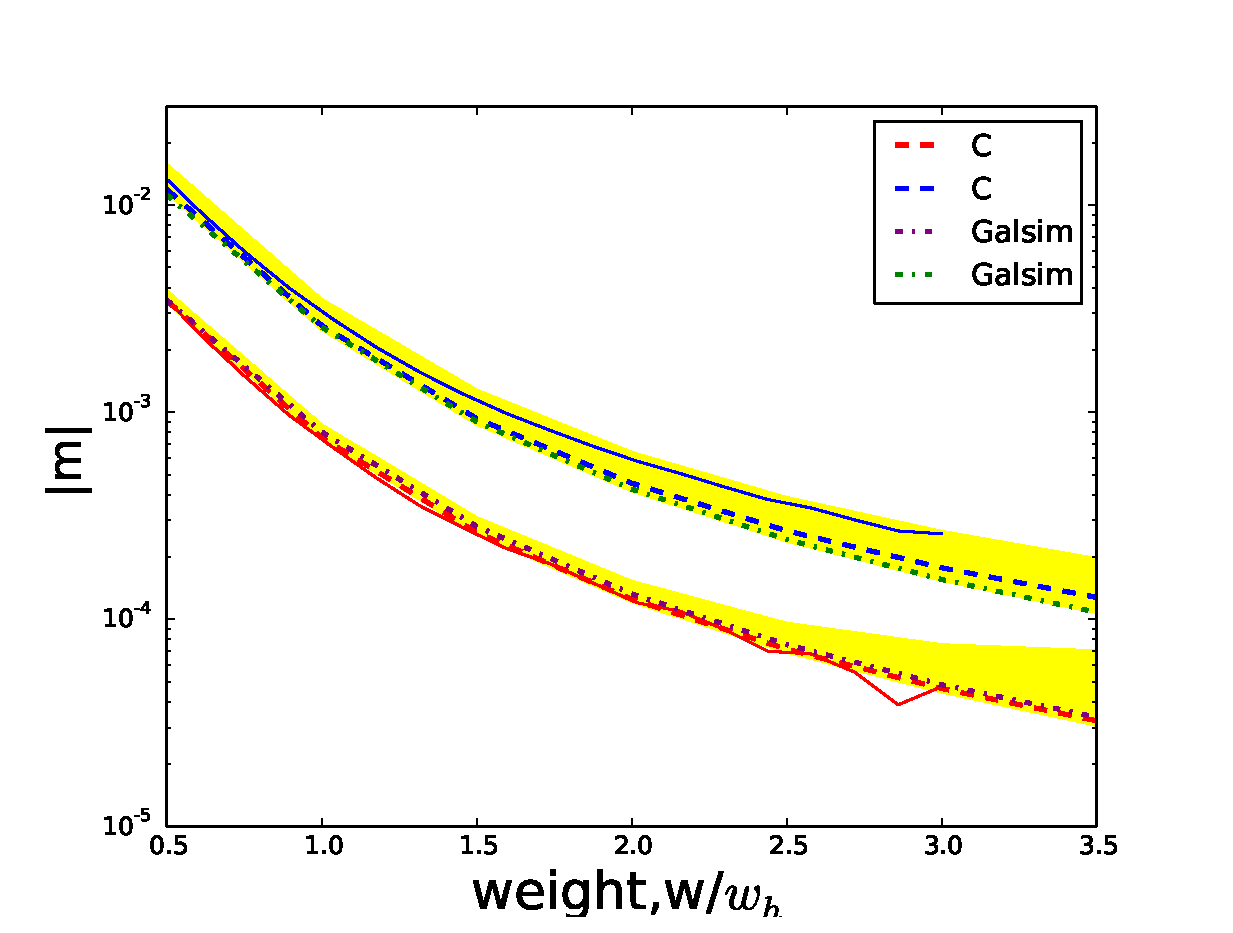
\includegraphics[width=\hsize]{cvsgalsim.eps}}
\caption{The CG bias in shear versus width of the weight function
(in units of the half-light radius $w_{\rm h}$) used to compute the
quadrupole moments.  The solid lines correspond to the results 
from \citetalias{Semboloni13} for the large (`B'; red) and small (`S'; blue) reference galaxy .
The dashed (dash-dotted) lines are our results for images
simulated using the C (GalSim) code.  {\bf We need to include a panel
  showing the differences with \citetalias{Semboloni13}.}}
\label{fig:biasofweight}
\end{figure}


\subsection{Calibration of CG bias using simulated HST images}
\label{sec:noisy}

The {\it Euclid} observations lack high-resolution multi-band images to measure
the CG bias directly. However, \citetalias{Semboloni13} showed that 

We outline the method that calibrate the CG bias using two bands
images, while the details can be found in \citetalias{Semboloni13}. We will use two narrow
band images to reconstruct the image at each wavelength. For each of
the narrow filter the image can be approximated by:
%
\be
I_i(\theta) = \int_{\Delta \lambda_i} T_i(\lambda)\, I(\theta,\lambda) \;\d \lambda,
\elabel{linearitp}
\ee
%
where $T(\lambda)$ is the transmission, and $i=1,2$ stand for the two bands.
We assume that for each pixel the image can be interpolated linearly:
%
\be
I(\theta,\lambda) \approx
I_{\rm inter}(\theta,\lambda)=a(\theta)\lambda + b(\theta).
\elabel{interpolate}
\ee
%
Eqs.\ref{eq:linearitp} and \ref{eq:interpolate} yield a linear set of
equations on each pixel, which can be used to solved for the
coefficients $(a,b)$:
%
\be
T_{ai} \lambda a(\theta) \,+\,T_{bi} b(\theta) = I_i(\theta), \quad\; i=1,2,
\elabel{lineareq}
\ee
%
where $T_{ai,\,bi}$ is the integrated transmission function at two
filters. With $(a,b)$ and Eq.\ref{eq:interpolate}, one can obtain
approximated galaxy images of each wavelength
$I(\theta,\lambda)$. Then we will follow the same procedure as in
previous section to estimate the CG bias.

The same two galaxy models from previous section are used in the
simulation, and we simulate the images in two HST filters: F606W,
F814W, which cover the filter of Euclid image survey. The spectra of
the galaxy are shifted according to their redshift, but the evolution
of the galaxy or the cosmology are not adopted in the simulation. The
spatial resolution is $0.05$ arcsec/pixel. The PSF is modeled by the
Airy function with diameter $D=2.5$ and obscuration $0.33$, which is
the configuration of HST. As shown in \citetalias{Semboloni13}, one needs to correct the
PSF effect in the observed images, or the CG bias will be
underestimated. We will adopt the same step: deconvolution for images
before the bias estimation and discuss that for the noisy images
later.

In order to see the effect of noise in the galaxy image, we add
Gaussian noise into the simulated HST images. An ideal level (SNR=50)
and a moderate level (SNR=15) are used to see the effect of the CG
bias. The RMS of the Gaussian image noise is determined by the total
flux ($F_{tot}$) within a certain radius $1.5\,r_h$
%
\be
\sigma = {F_{tot} \over {\rm SNR} \sqrt{N_{tot}} },
\ee
%
where $N_{tot}$ is the total pixel number within $1.5\,r_h$.  In
Fig.\ref{fig:ests2n}, we compare the input SNR with that estimated by
SExtractor \citep{1996A&AS..117..393B}. We can see that the
estimations are slightly higher than the input values at $SNR=15$, but
still within a reasonable value for real weak lensing survey.
%
\begin{figure}
\centerline{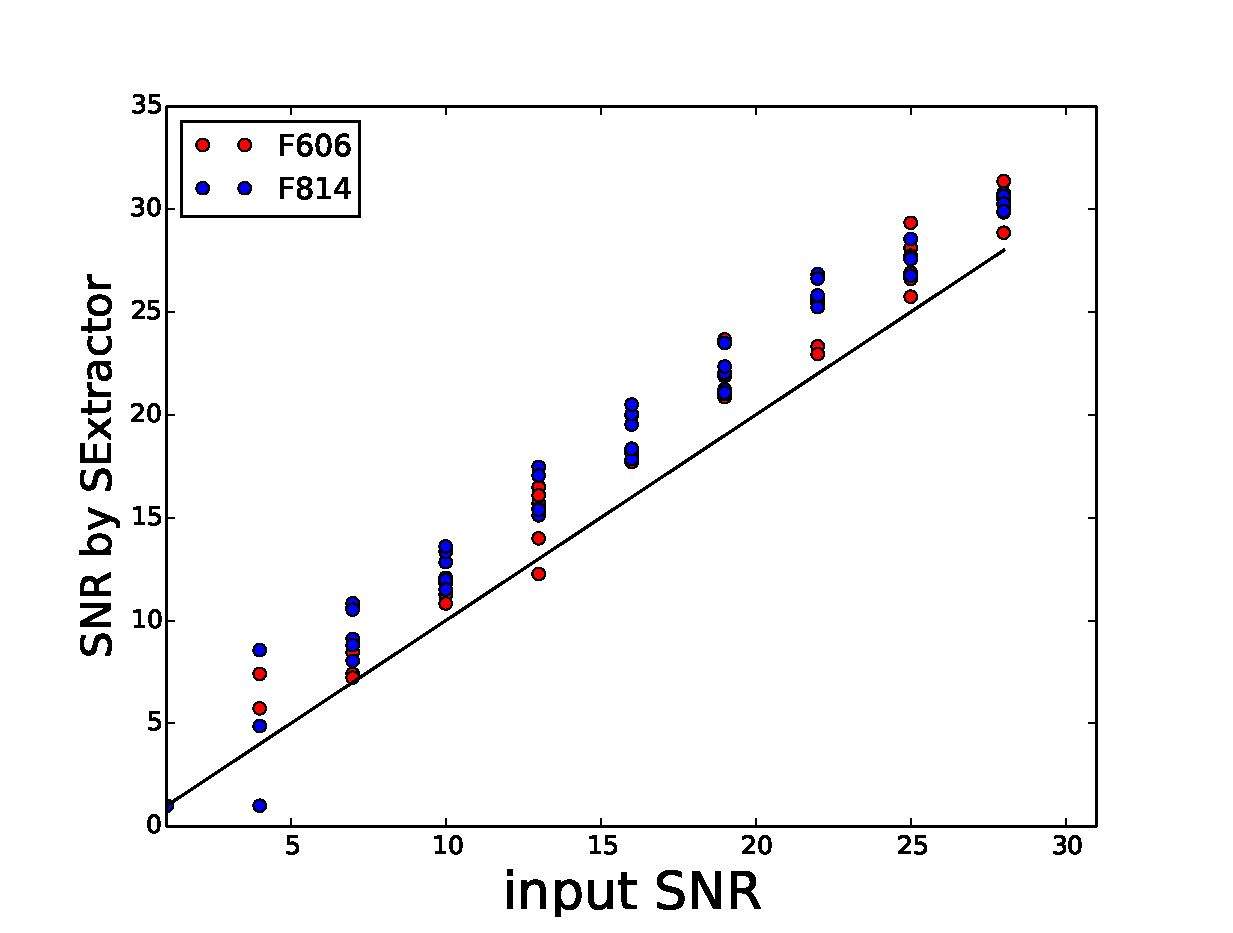
\includegraphics[height=5cm,width=5.0cm]{zs2ncB.eps}
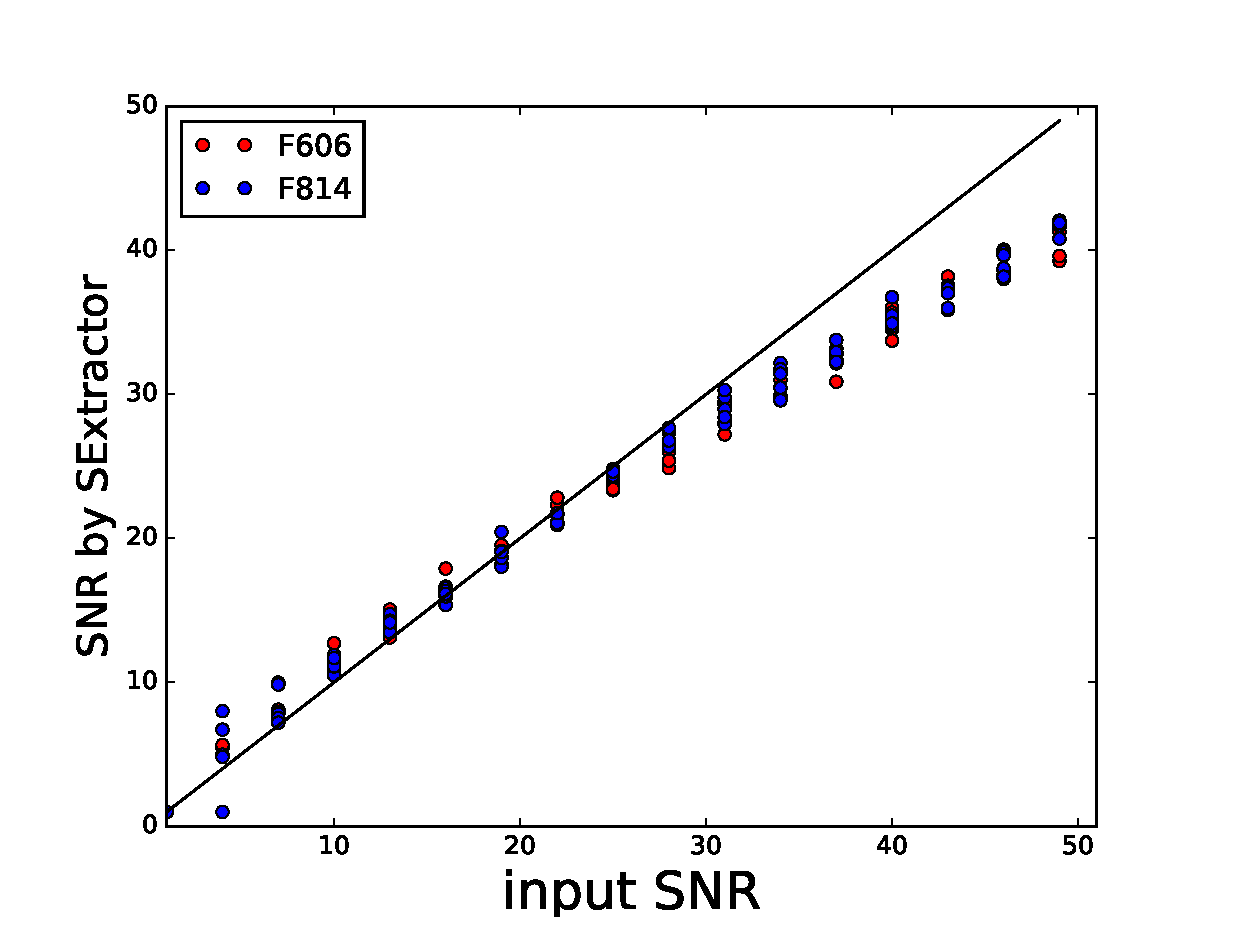
\includegraphics[height=5cm,width=5.0cm]{zs2ncS.eps}}
\caption{SNR estimated by SExtractor vs input SNR. Left is for the
  B-galaxy; Right is for the S-galaxy.}
\label{fig:ests2n}
\end{figure}
%

Direct devonvolution of a noisy image will end with a strange galaxy
image and large numerical noise, thus we apply Galfit
\citep{2010AJ....139.2097P} to fit the noisy image, and use the fitted
image as our noise reduced observed image, i.e. the residual noise is
not taken into account for CG analysis. For the necessary fitting
profile and number of components, we also use two Sersic components as
bulge and disk for both image bands. For each image, we apply further
constraints to the galaxy parameters: Sersic index, effective radius,
and axis ratio (Table \ref{fitpar}).
%the effective radius can be achieved at a small variations (within
%$20\%$), while the Sersic index usually has a large difference from
%the input values as well as scatter.

In order to provide a initial parameters for Galfit, we use the
stacked image of two bands to estimate the center and some initial
values of the galaxy parameters from SExtractor. The fitting images
slightly depend on the initial values, and can change the estimate for
the CG bias estimation. The dependence will become significant with
the decreasing of image SNR. In the following estimation for the CG
bias, we will perform the image fitting using two kinds of initial
parameters: in the first one we will leave all the fitting parameters
free; while in the other one we will freeze the Sersic index as the
simulated value, and leave the others free. As we will present,
with sufficient large samples, the estimation using noisy images for the
CG bias can converge, and is independent of the initial parameters.

%
\begin{center}
\begin{table}
\begin{tabular}{|c|c|c|c|c|}
\hline\hline
 &S-606W  & S-814W  & B-606W & B-814W \\ \hline
$n_1$ &0.5-2.5  &0.5-2.5  &0.5-2.5 &0.5-2.5 \\ \hline
$n_2$ &0.5-2.5  &0.5-2.5  &0.5-2.5 &0.5-2.5 \\ \hline
$R_{bulge}$ &1-10 &1-10  &3-30  &3-30  \\ \hline
$R_{disk}$  &5-30 &5-30  &10-60 &10-60 \\ \hline
$q$      &0.6-1  &0.6-1  &0.6-1 &0.6-1 \\ \hline
\hline
\end{tabular}
\caption{\label{fitpar} Constraints for the fitting parameters in Galfit.
The first two columns are for two images of the S-galaxy, the other two are
the image of B-galaxy.
$n_1$ is the Sersic index for bulge, and $n_2$ is the Sersic index for disk.
The effect radius is given in unit of pixel ($0.05$ arcsec).}
\end{table}
\end{center}
%
%\begin{figure}
%\centerline{\includegraphics[width=7.0cm]{zsnrre.eps}
%\includegraphics[width=7.0cm]{zsnrn.eps}}
%\caption{The fitting parameters (Sersic index and effect radius).}
%\end{figure}

Applying the calibration method to the fitted images, we can obtain
the estimation of the CG bias for the simulated images. In
Figs.\ref{fig:biasofz50} and \ref{fig:biasofz15}, we show the shear CG
bias with redshift. In each panel, we show different estimates for the
bias:
\begin{itemize}
\item
The black solid lines are the ``True'' CG bias: we use the true
SED of the galaxy and images of each wavelength to estimate the bias
without approximation.
\item
The dashed lines are the estimation using two
HST images without noise.
\item
The colour lines are those using noisy images. The difference between
red and blue lines are in the image fitting: for the red lines, we
free all the parameters in image fitting, for blue lines we fix the
Sersic index as the input value. For the orange lines we also free all
the parameters, but we perform another convolution with the effective
PSF (see appendix for more detail). In Fig.\ref{fig:flowchart} one can
see that the convolution is canceled with the last deconvolution for
the CG images.  The reason for that is the deconvolution may cause
some numerical errors, especially for the small size noisy images. The
extra PSF convolution will not significantly change the CG bias as we
will show in the appendix. Therefore, in the following result for
noise images, we will perform the convolution to the NCG image instead
of deconvolution to the CG one.
\end{itemize}
Moreover, although we use the circular source image in the simulation,
the fitted noisy images will become slightly elliptical. In order to
get rid of the error due to the ``intrinsic shape'', we rotate the
source image $6$ times, and use the average value as our estimate for
the galaxy ellipticity \citep{2007AJ....133.1763N}. At each redshift,
we use one noise free image and $40 (200, 300)$ noisy images for $SNR=50
(SNR=15)$.  In the bottom panel of each figure, we also show the
residues with respect to the true CG bias, and the error bars, which
are given by the standard deviation from $e_{cg}$ and $e_{ncg}$
%
\be
\sigma_m= |m| \sqrt{\rund{\sigma_{cg} \over \langle e_{cg}\rangle }^2
  + \rund{\sigma_{ncg} \over \langle e_{ncg} \rangle}^2 }.
\elabel{sigmam}
\ee
%
In the error panel, the grey shadow stands for the error budget of CG
bias in Euclid cosmic shear analysis \citep[$\pm
  0.00025$][]{2013MNRAS.431.3103C,2013MNRAS.429..661M}.

One can see that in general our estimate can reproduce the properties
of CG bias in ellipticity measurement using both ideal or noisy
images.  In the high SNR cases (Fig.\ref{fig:biasofz50}), all the
estimates with different initial parameters basically agree with each
other. The estimate with all fitting parameters free gives lower bias
than that fixed the Sersic index. In the low SNR case
(Fig.\ref{fig:biasofz15}), the fitting using all free parameters show
better estimates for the CG bias, and the residual are within the
requirement for most cases. The variance due to the image fitting with
different initial parameters are larger than high SNR cases, but can
still be reduced by large sample of images and reach the requirement.
It means that for each single type of galaxy, one need about $300$
galaxy images in order to calibrate the bias. The scatters in the
estimation are proportional to the magnitude of the bias, i.e. we have
large uncertainty for S-galaxy at low redshift. We also perform tests
using images with lower SNR, and calculate the average residue with
respect to true bias. When the SNR of images drop to $12$, the average
residue increases by about $70\%$($60\%$) for small(big) galaxy than
that of SNR$=15$. This test may not reflect the real dependence on the
SNR of images, since in general the lower SNR, the smaller the image
size. Therefore, image simulation with specific configuration of the
survey is necessary, e.g. the limit magnitude, the population of the
galaxies and the relation between the size and SNR etc.
%(from $0.00015$ to $0.00027$, 9.9e-5 to 0.00016).
%%%%%%%%%%%%%%%%%%%%%%% method dependence
In additional tests using other measurement methods for PSF
correction, such as the image fitting methods
\citep[e.g.][]{2007MNRAS.382..315M,2008MNRAS.390..149K,2013MNRAS.429.2858M},
and KSB+ \citep[e.g.][]{1998ApJ...504..636H,2006MNRAS.368.1323H}, we
find that the bias has similar dependence on the SED of the galaxies,
but with different amplitude.

In both two figures, we notice that at $z=0.5$ and $0.9$, the estimates are
significantly smaller than the true bias for both galaxy models. This is
due to the uneven SED of the source galaxy in the two HST filter. In
Fig.\ref{fig:sedz}, we compare the SED of the galaxy in redshift
$z=0,0.5$. One can see that at $z=0.5$, besides the strong emission
lines, the linear approximation cannot reflect the properties of the
source galaxies. Thus for some galaxies with complex properties, two band
image may not be sufficient to calibrate the CG bias.
%In Fig.\ref{fig:err2snr}, we show the average residual bias
%$\bar{|m|}$ over the redshift as a function of SNR of the images. For
%each SNR, we average the residual in redshift range from $0$ to $1.2$,
%and for each redshift, $50$ noise realizations are used. One can see
%that for the images with SNR smaller than $\sim10$, the errors of our
%estimate will be non negligible, and the estimation thus cannot
%provide trustable calibration. Another simplification that we adopt
%here is that the SNR we used in two bands are the same. This is in
%reality not the case in most the time. In the more sophisticated
%simulation, the image SNR of two bands need to be determined by the
%colour of the galaxy.
%%%%%
\begin{figure}
  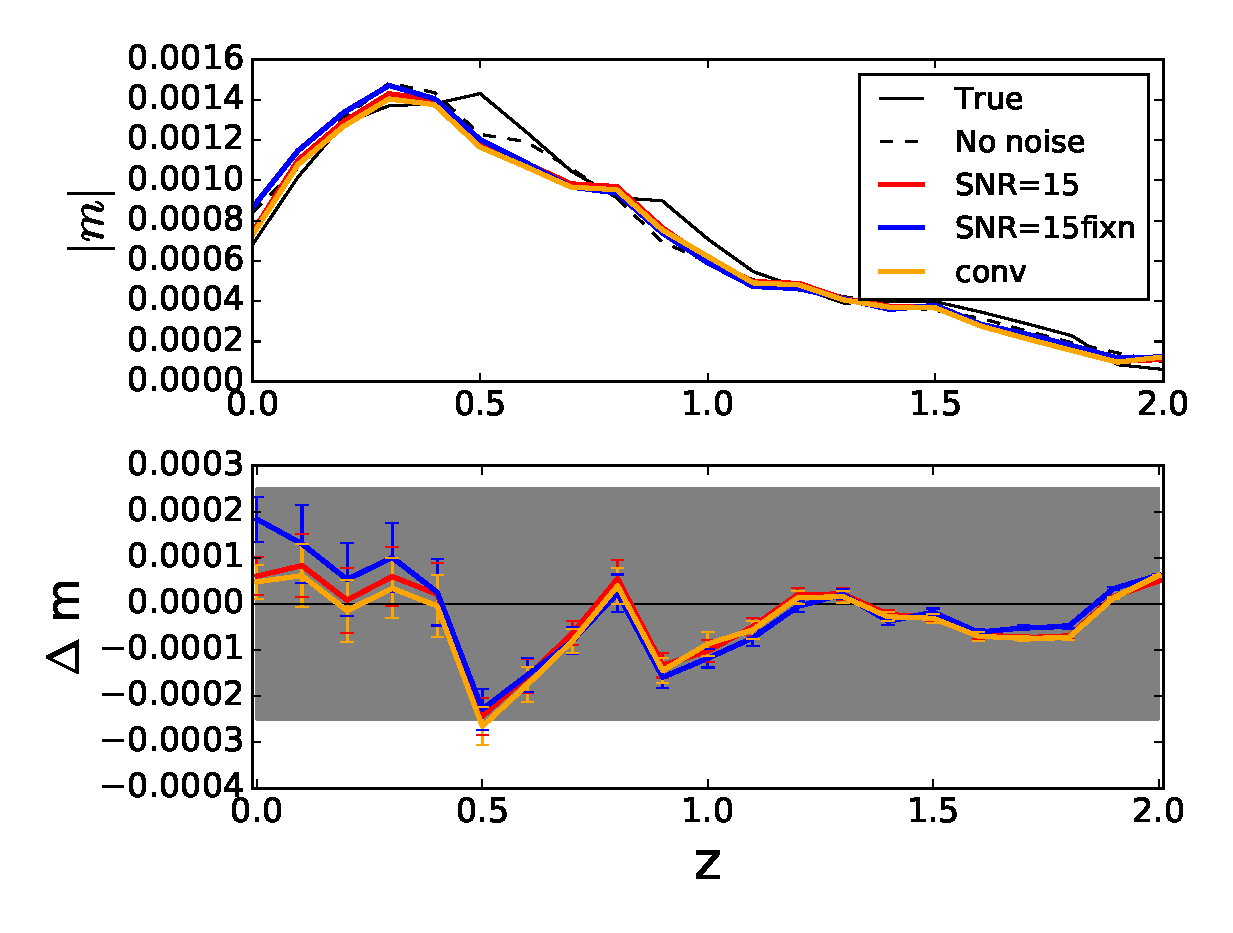
\includegraphics[width=8.0cm]{zs2n_b_snrtt50.eps}
  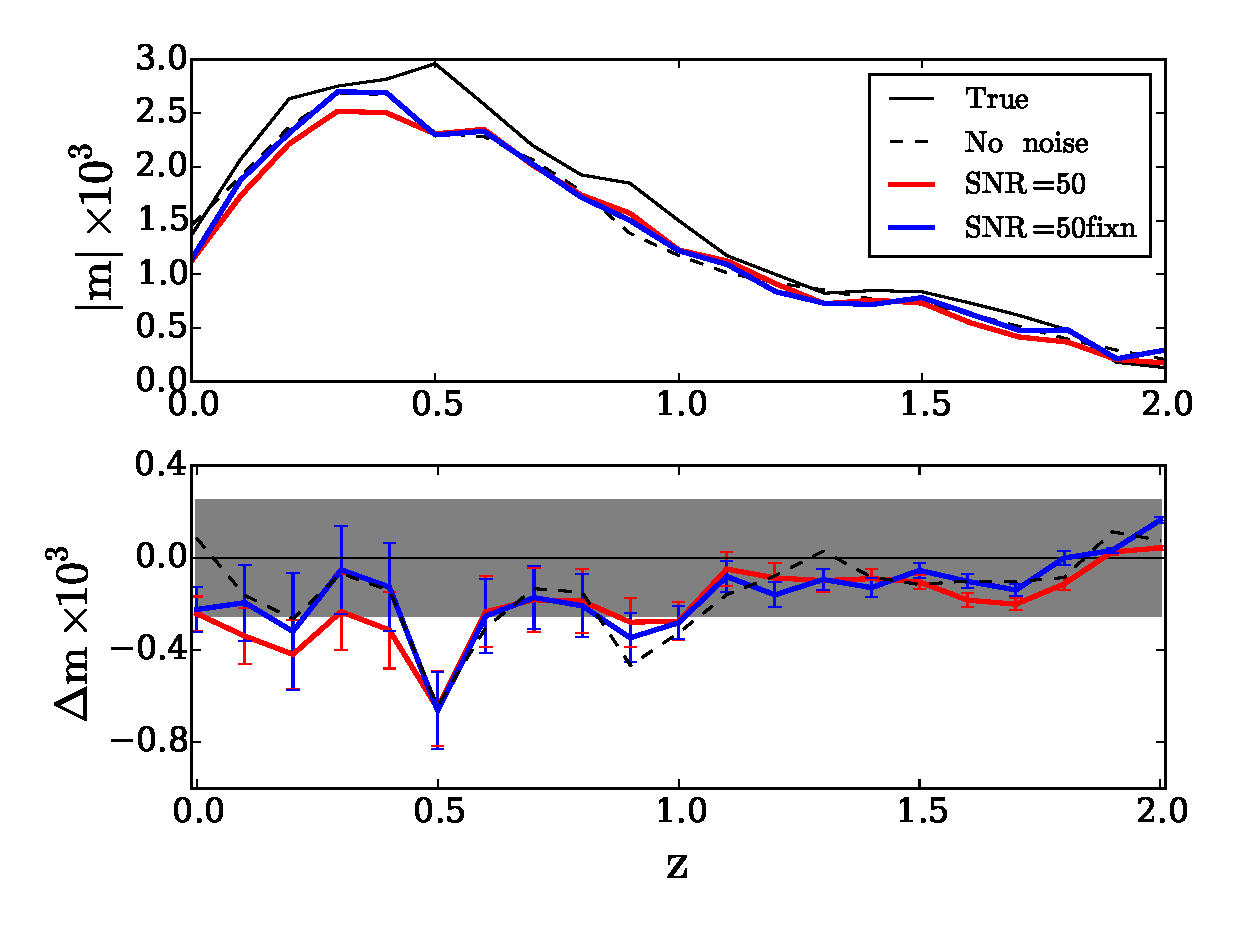
\includegraphics[width=8.0cm]{zs2n_s_snrtt50.eps}
\caption{The CG bias in shear measurement as a function of redshift
  using simulated images. The black solid lines are the true CG bias;
  the dashed lines are the estimation using two band HST images
  without noise; the colour lines are the estimation using noisy
  images of input $SNR=50$, the value are the average over $40$
  realizations each redshift. In the bottom, $\Delta m$ is the
  residual with respect to the true CG bias, and the error bars show
  the standard variations (Eq.\ref{eq:sigmam}). $Up(Down)$-figure are
  the results for B-(S-)galaxy.}
\label{fig:biasofz50}
\end{figure}
\begin{figure}
  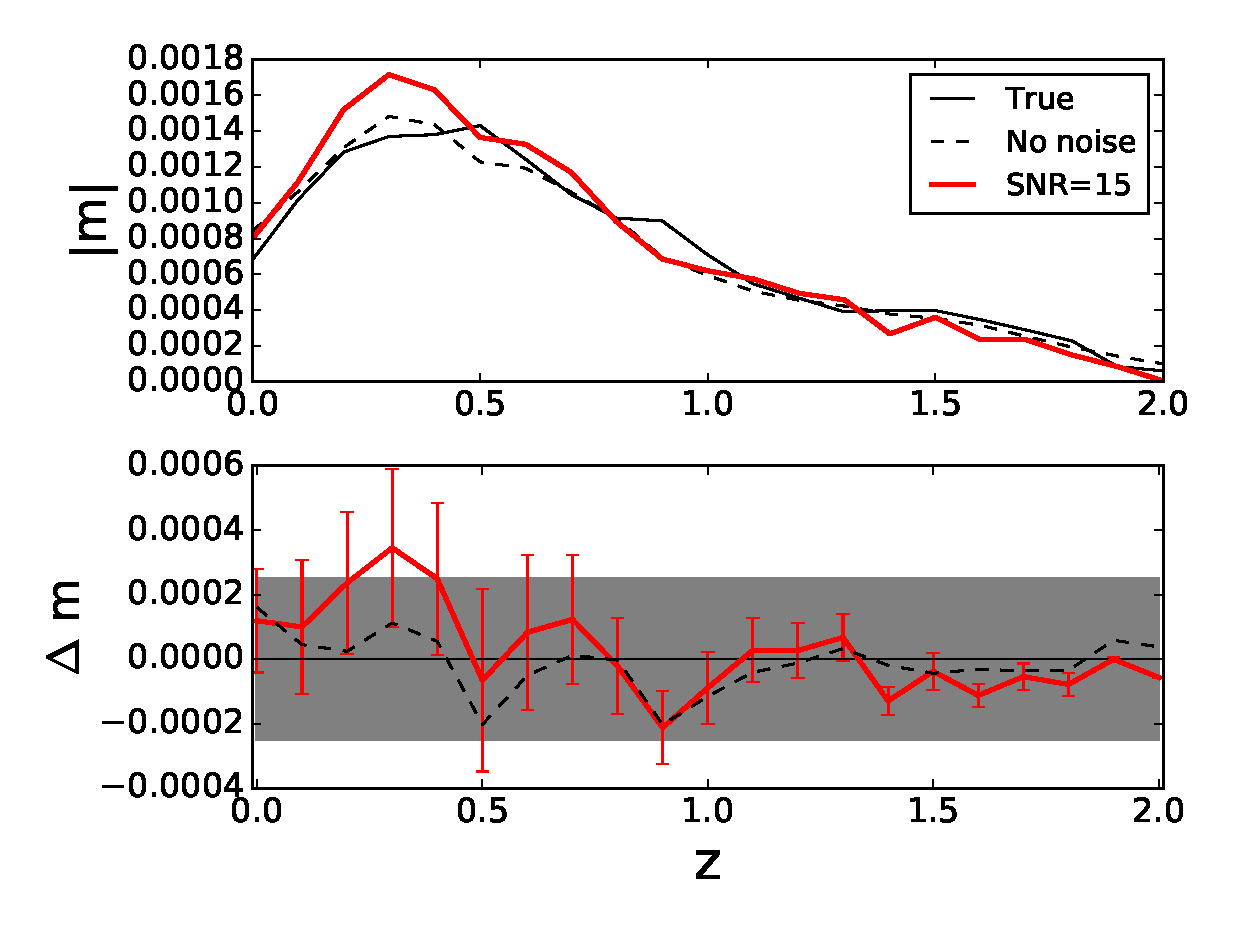
\includegraphics[width=8.0cm]{zs2n_b_snrtt15.eps}
  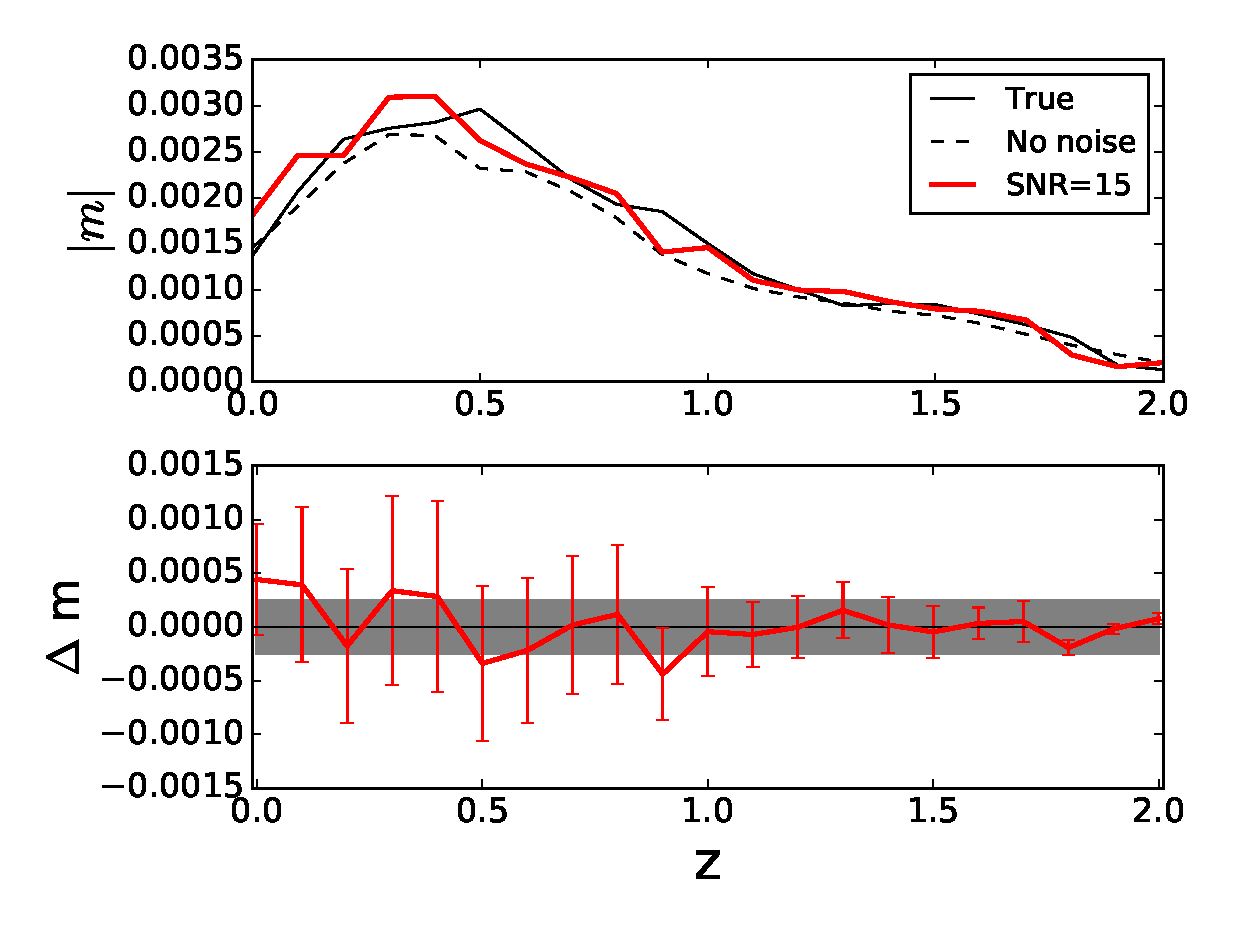
\includegraphics[width=8.0cm]{zs2n_s_snrtt15.eps}
\caption{Same as Fig.\ref{fig:biasofz50} but for images of SNR=15.
  $200$ realizations are used for the red lines at each redshift and
  $220$($320$) realizations are used for blues lines for the
  B-(S-)galaxy. }
\label{fig:biasofz15}
\end{figure}
%
\begin{figure}
\centerline{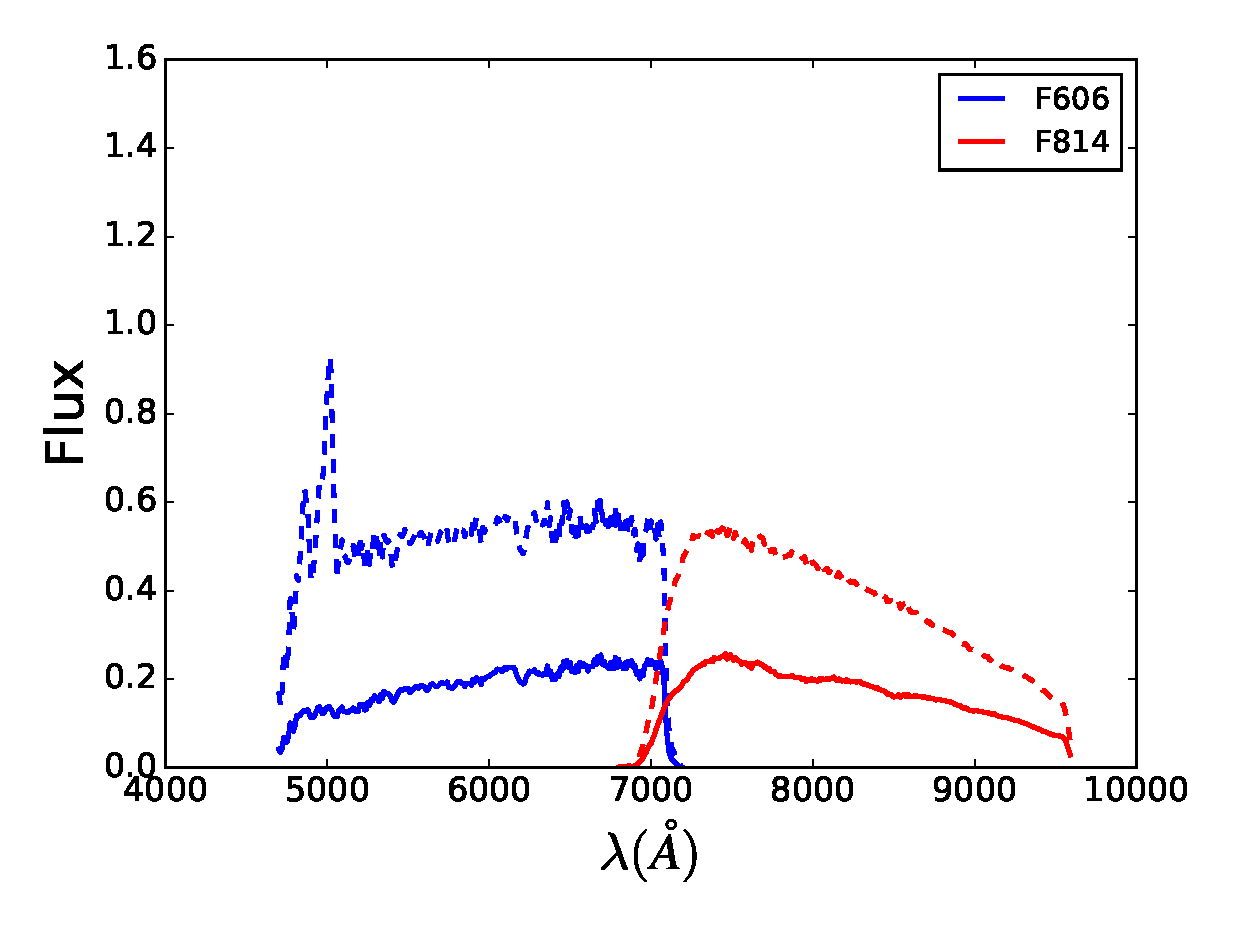
\includegraphics[width=4.0cm]{z0bandsed.eps}
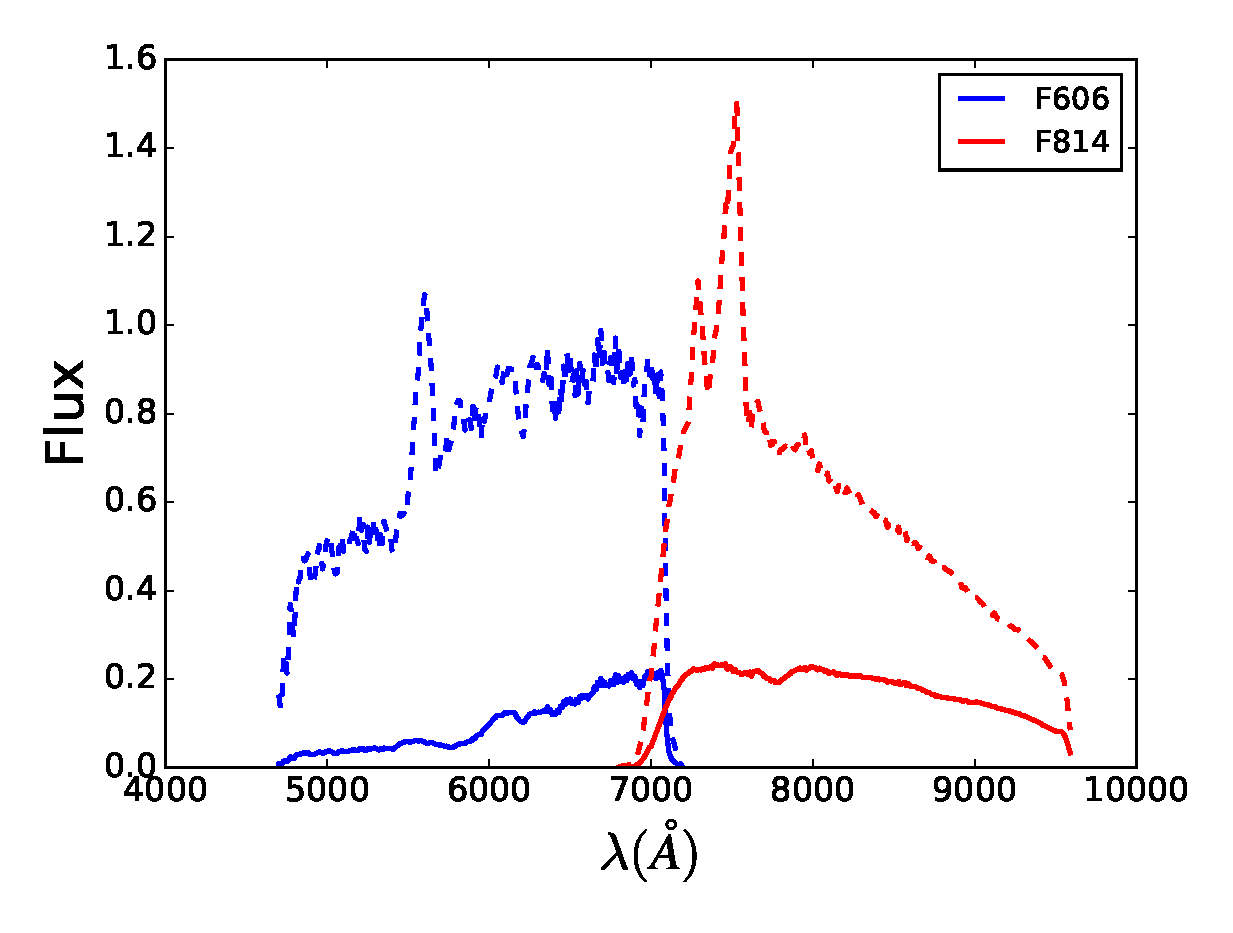
\includegraphics[width=4.0cm]{z5bandsed.eps}}
\caption{Spectral energy distributions used to create the disc and
  bulge components of our mock galaxies. They are normalized at
  $\lambda=5500$\AA$\,$ by ratio $F_{\rm bulge}/F_{\rm disk}=1/3$, and they
  are convolved with HST filter function in F606W and F814W. $left$-
  redshift $0$; $right$- redshift $0.5$.}
\label{fig:sedz}
\end{figure}

\subsection{PSF variations in calibration data from HST}

In the previous test, we used an ideal circular symmetric Airy PSF
model. It may however cause inaccuracy in our estimation of the CG
bias. Thus, we perform additional tests due to the variations of the
PSF. The noise free images are used in order to isolate the effects of
the PSF. The different PSF models are applied only in the step of
deconvolution for the simulated HST images.

First we generate three pairs of PSF model by slightly increasing the
size of PSF. The effect on the CG bias is shown in
Fig.\ref{fig:psfacc1}. From solid, dashed to dotted lines, we
increased the PSF size of the F606 bands; while from red, green to
blue lines, we increase the PSF size of the F814 bands. Although the
effect due to the two PSF variations depends on the SED of the source
galaxy, one can see that increasing the size of the PSF in different
bands will cause either on increase or decrease in the CG bias
calibration. Once again, we can see that the small galaxies are more
sensitive to the variation of PSF.

To test the impact of imperfect PSF modelling, we make two
comparisons: Comparing a control set of ``actual'' PSFs to a mock set
of stars using these PSFs, including some unresolved binaries; and
comparing the stars in actual images to the best-fit models. In the
former case, we generate mock star fields using PSFs generated with
the TinyTim tool \citep{2011SPIE.8127E..0JK} and allow 30 per cent of
stars to be unresolved binaries, with another star laid on top of them
within a radius of one pixel. In the latter case, we use actual star
fields observed with HST and try two methods of fitting the model to
the stars. In both cases. we perform this for both the F606W and F814W
filters.

The model PSFs are generated using the default parameters for TinyTim
where possible, and the appropriate camera, detector, and filter
passband settings for each image. For the rest of the options, we use:
\begin{itemize}
  \item \textbf{Position on Detector:} Chosen for each star based on its
detected position.
  \item \textbf{Spectrum:} 1; 15 (Use the K7V spectrum, which is chosen
to represent a typical star in the sample. The choice of a fixed
spectrum for stars was found to have a negligible impact on the
models.)
  \item \textbf{PSF Diameter:} 2.0 arcsec
  \item \textbf{Focus-Secondary Mirror Despace:} Fit per image. As HST
    ``breathes'' due to its varying angle relative to the Sun, the
    position of the focus relative to the secondary mirror changes
    over time and cannot be perfectly predicted for any given
    observation. We thus have to fit the best focus position by
    simulating multiple sets of PSFs for each image.
  \item \textbf{Zernike Polynomials:} In the first test, ``focus
    only'', set to default values. In the second test, ``all
    parameters'', these are fit in addition to the focus despace.
  \item \textbf{Subsampling Factor:} $8\times$
\end{itemize}

Stars are selected such that they have a signal-to-noise ratio of at
least $50$, there are no detected objects within $1$ arcsecond ($20$
pixels), and outlier rejection is performed in the fitting procedure.
The stars are normalized and then stacked using inverse-variance
weighting. The corresponding model PSFs are stacked using the same
weights.

%
\begin{figure}
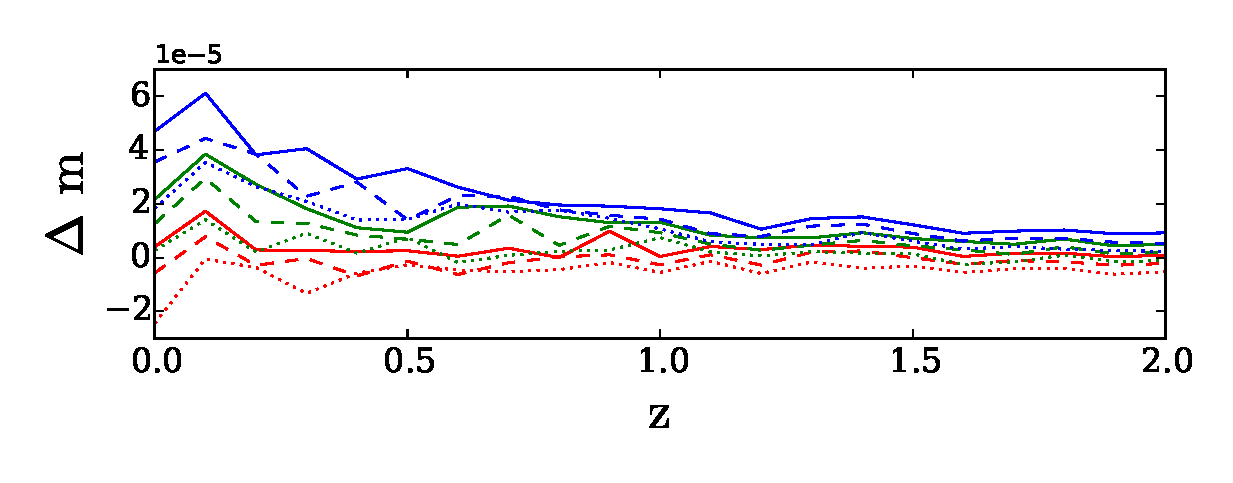
\includegraphics[width=8.0cm]{varpsfB.eps}
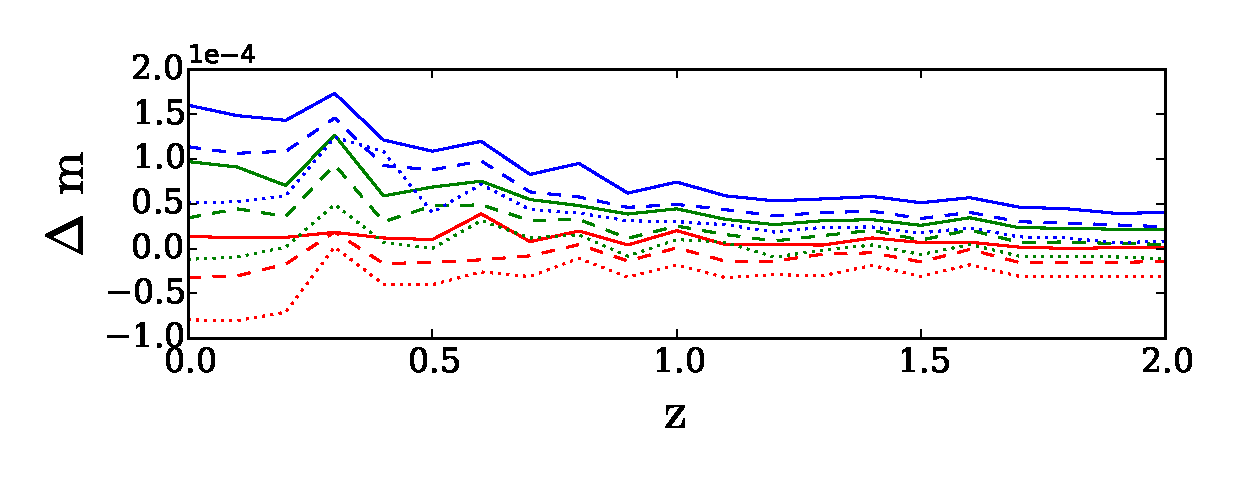
\includegraphics[width=8.0cm]{varpsfS.eps}
\caption{The PSF in the deconvolution are varied to see the effect on
  the CG bias.  From red, green to blue lines, we increase the size of
  PSF for the F814W; from the solid, dashed to dotted lines we
  increase the size of PSF for the F606W.  }
\label{fig:psfacc1}
\end{figure}
%
\begin{figure}
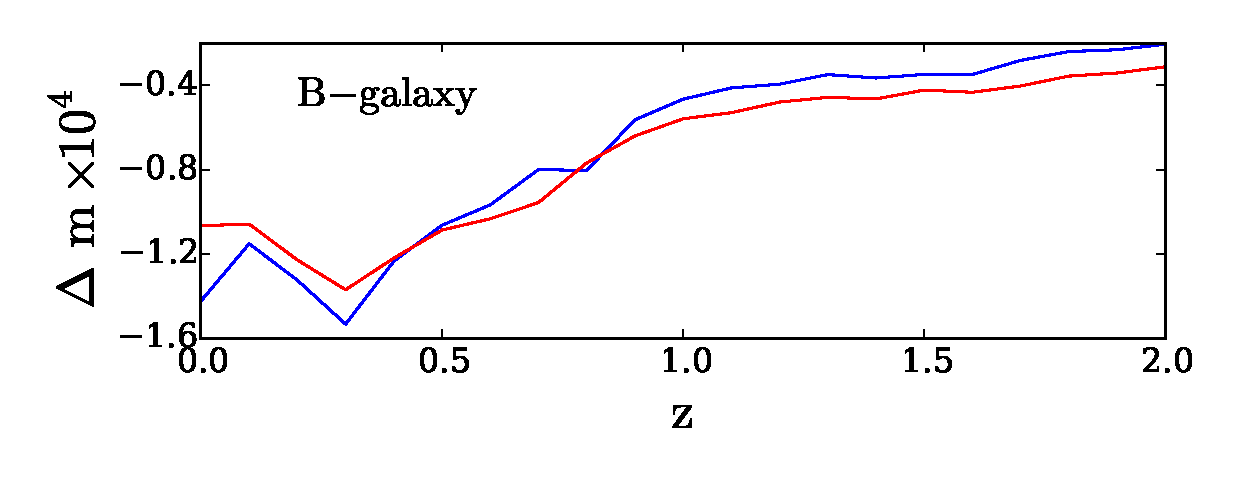
\includegraphics[width=8.0cm]{ztinytim_b.eps}
%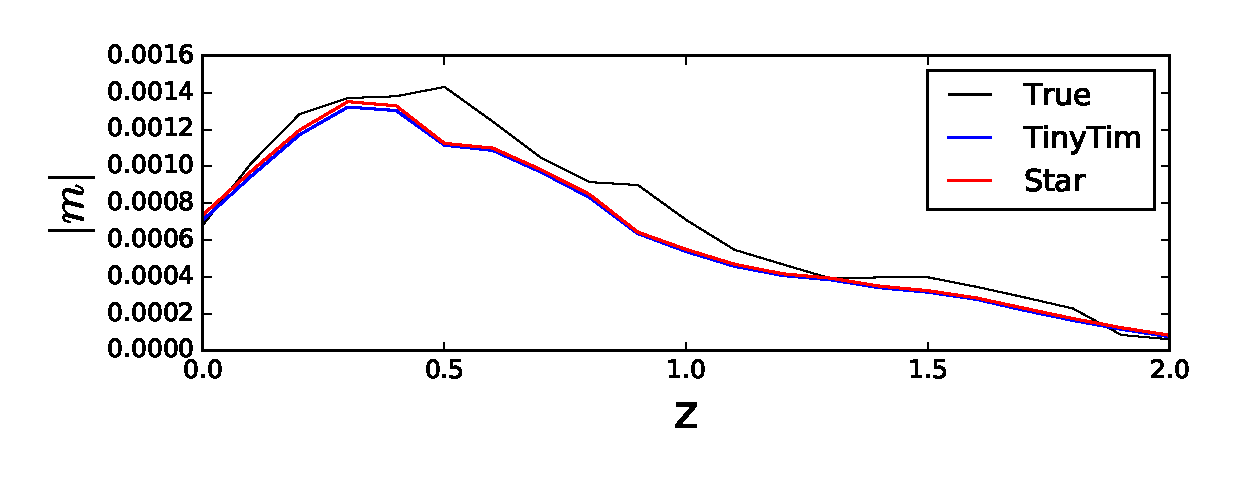
\includegraphics[width=8.0cm]{z_b_bryan2.eps}
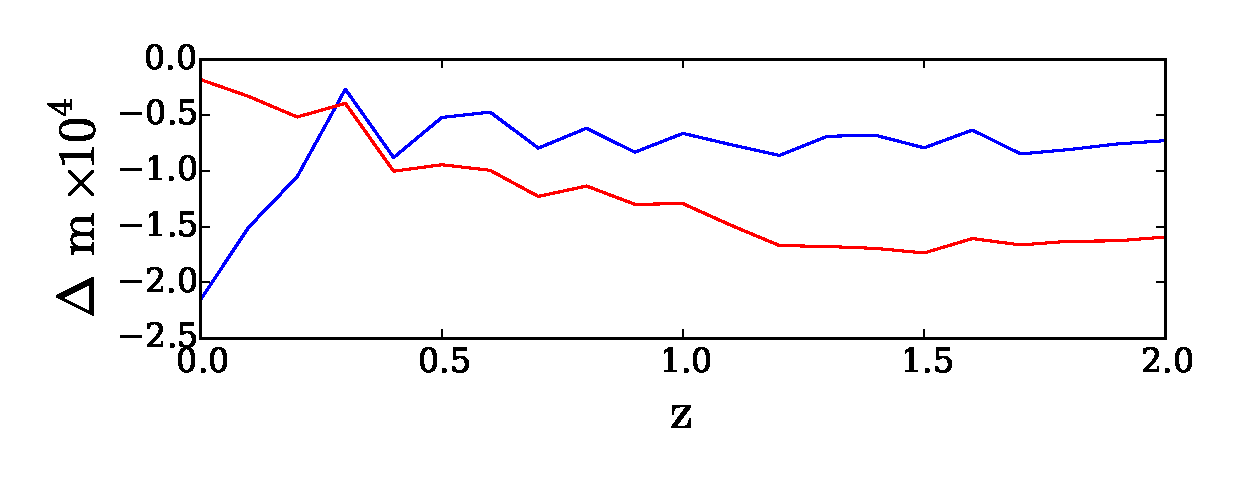
\includegraphics[width=8.0cm]{ztinytim_s.eps}
%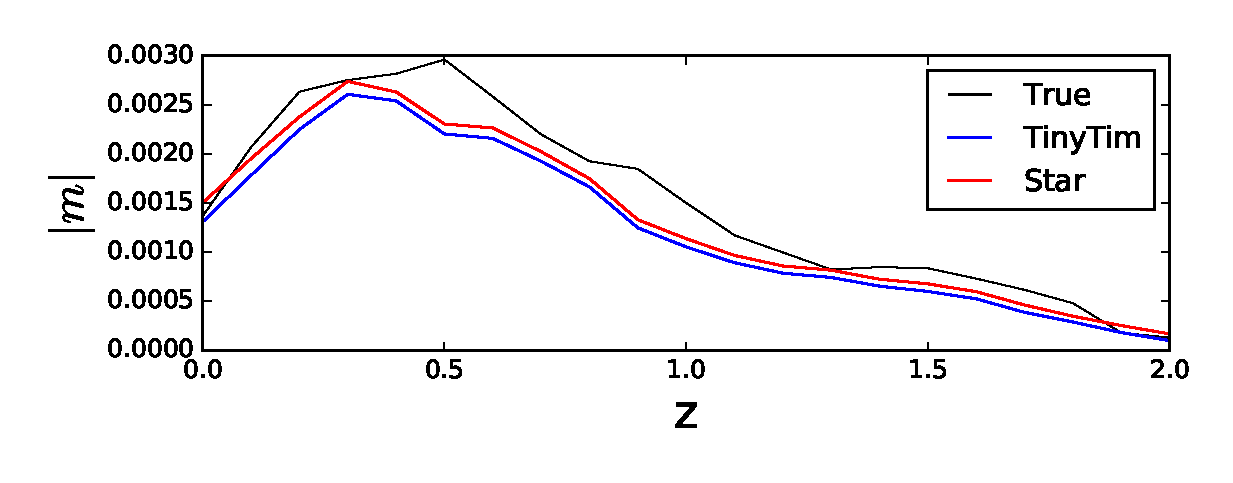
\includegraphics[width=8.0cm]{z_s_bryan2.eps}
\caption{Comparison of PSF between TinyTim model and stars.
  Top (Bottom) is for the B-galaxy (S-galaxy). The solid (dashed) 
  lines are the result using undrizzled (drizzled) PSF. 
  The dotted lines are that if we also include binary PSF effect.}
\label{fig:psfacc2}
\end{figure}
%
In Fig.\ref{fig:psfacc2}, one can see that the inaccuracy of PSF can
cause error on the estimation of CG bias. For the small size galaxy,
the error can reach about $15\%$ for undrizzled PSF, while for the big
galaxy, the error is only a few percent, can be neglect. In the result
using drizzled PSF, the difference becomes smaller. The most
problematic PSF will be those from binary stars. One can see for both
big and small galaxies, we have a significant error.

\section{CANDELS data}
\label{sec:candels}

\subsection{Calibration sample}
In this section, we use the real galaxy images to estimate the CG bias
which will appear in the Euclid weak lensing survey. For the reference
PSF of Euclid, we use the Airy model (Eq.\,\ref{eq:psfairy}), and we use
the PSF model from TinyTim for the HST data.

To investigate the impact of colour gradients using realistic galaxies
populations, we employ HST/ACS data taken in the F606W and F814W
filters in the three CANDELS fields (AEGIS, COSMOS, and UDS), which have
a roughly homogeneous coverage in both bands
\citep[see][]{davis2007,grogin2011,koekemoer11}. We base our analysis
on a tile-wise reduction of the ACS data, incorporating pointings
which have at least four exposures to facilitate good cosmic ray
removal, yielding combined exposure times of 1.3-2.3ks in F606W and
2.1-3.0ks in F814W.  We employ the updated correction for
charge-transfer inefficiency from \cite{massey2014},
\texttt{MultiDrizzle} \citep{koekemoer2003} for the cosmic ray removal
and stacking, as well as careful shift refinement, optimised
weighting, and masking for stars and image artifacts as detailed in
\cite{schrabback2010}.  Schrabback et al. (in prep.) describe the
generation of weak lensing catalogues for these images.  We base our
analysis on the galaxies passing their source selection and apply
additional magnitude cuts as detailed below. To investigate the
dependence of the colour gradient influence on galaxy colour and
redshift, we match this galaxy catalogue to the photometric redshift
catalogue from \cite{skelton14}.  We list the total non-masked areas
in which these catalogues overlap in Table \ref{table:mag}.


We match the galaxy from V(F606W) and I(F814W) bands by selecting that
the difference of galaxy coordinates in two bands is smaller than 1
pixel ($0.05$ arcsec). Moreover, in order to resemble the Euclid image
survey, we apply selection based on the magnitude of two bands. In the
first selection, the galaxy must be brighter than magnitude $25$ in
V-band and $24.5$ in I-band. In the second selection (VIS, N2 sample),
we apply the linear interpolation from V and I band using the
effective wavelength to approximate the Euclid VIS magnitude, and
select the galaxy brighter than $24.5$ in VIS. In the last one (N3
sample), we enlarge the sample by using lower threshold in two bands:
$25.5$ in V and $25.0$ in I band. The amount of galaxies is listed in
Table\ref{table:mag}.
%
The galaxy VIS magnitudes will determined by several factors, such as
exposure time and filter transmission, etc. Thus, the actual number of
galaxies can be different from what we have shown in this work. The
approximation that we use rely on the flatness of the source
spectrum. In the VIS sample, the number of galaxies is similar to that in
the first selection in all three fields, which suggest that the
spectra of our galaxies are relatively smooth. In the N3 sample the galaxy
number is much higher.
%
The total galaxy number and number density ($\sim$12/arcmin$^2$) is
lower than that in \citetalias{Semboloni13} for several reasons: the galaxies are selected
which the 3D-HST photometric redshift are available, and those
suitable for weak lensing analysis, e.g. the very big or bright
galaxies are not include. Moreover, in \citetalias{Semboloni13} the galaxies are selected
by the magnitude of F814W. However we select galaxies by the estimated
VIS magnitude and well match in F606W and F814W.

There is no significant difference found in the distribution of galaxy
parameters, such as effective radius, axis ratio, photometric redshift
and colour (we use $m_{F606}-m_{F814}$ as colour in this work, and
will write as $m_{V-I}$ later). The SNR of most images in VIS sample
are larger than $15$, thus they will be able to provide relatively
stable estimate for CG bias.
%while the low SNR images may suffer from large uncertainty of bias estimation. Thus we only show the result in the VIS sample.

We also compare the galaxies from 3 catalogues (AEIGS, COSMOS, UDS).  In
the distribution of galaxy parameters (Fig.\ref{fig:datapro1}), we
find no significant difference in half light radius ($r_h$), galaxy
axis ratio or redshift distribution. However, in the colour
distribution, there are more blue galaxies (small $m_{V-I}$) in AEGIS,
which is more significant in N3 sample. We will see later that the
colour of galaxy is also related to the CG bias in shape measurement.
%There is slight difference in the SNR of two filters: the SNR of galaxies in AEGIS are larger than the other two in V-band, while smaller in I-band.
%
\begin{center}
\begin{table}
  \begin{tabular}{lllll}
    \hline
    Field   &Area (arcmin$^2$) &$N_1$ &$N_2$ &$N_3$\\
    \hline
    AEGIS   &180   &2094  &2112  &3460\\
    COSMOS  &139   &1593  &1656  &2449\\
    UDS     &146   &1455  &1497  &2341\\
    Total   &465   &5142  &5265  &8250\\
    \hline
  \end{tabular}
  \caption{\label{table:mag} Size of the HST CANDELS data sample in F606W
    and F814W bands.  The number of galaxies are shown in three selection
    methods to match the Euclid survey, $N_1$: $m_V<25$ and $m_I<24.5$,
    $N_2$: $m_{VIS}<24.5$, $N_3$: $m_V<25.5$ and $m_I<25$. }
\end{table}
\end{center}
%
\begin{figure*}
  \centerline{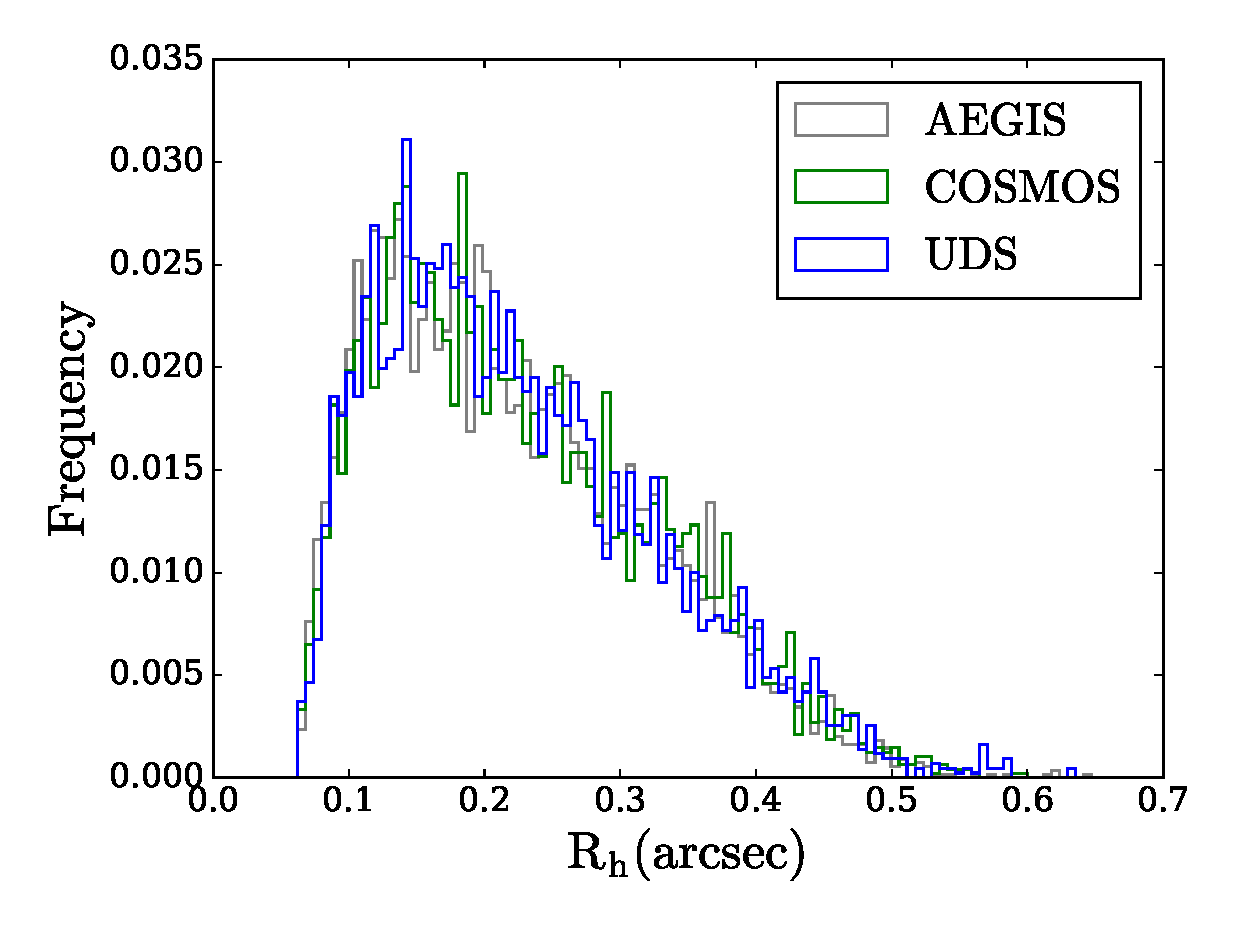
\includegraphics[width=5.0cm]{zhisrh.eps}
    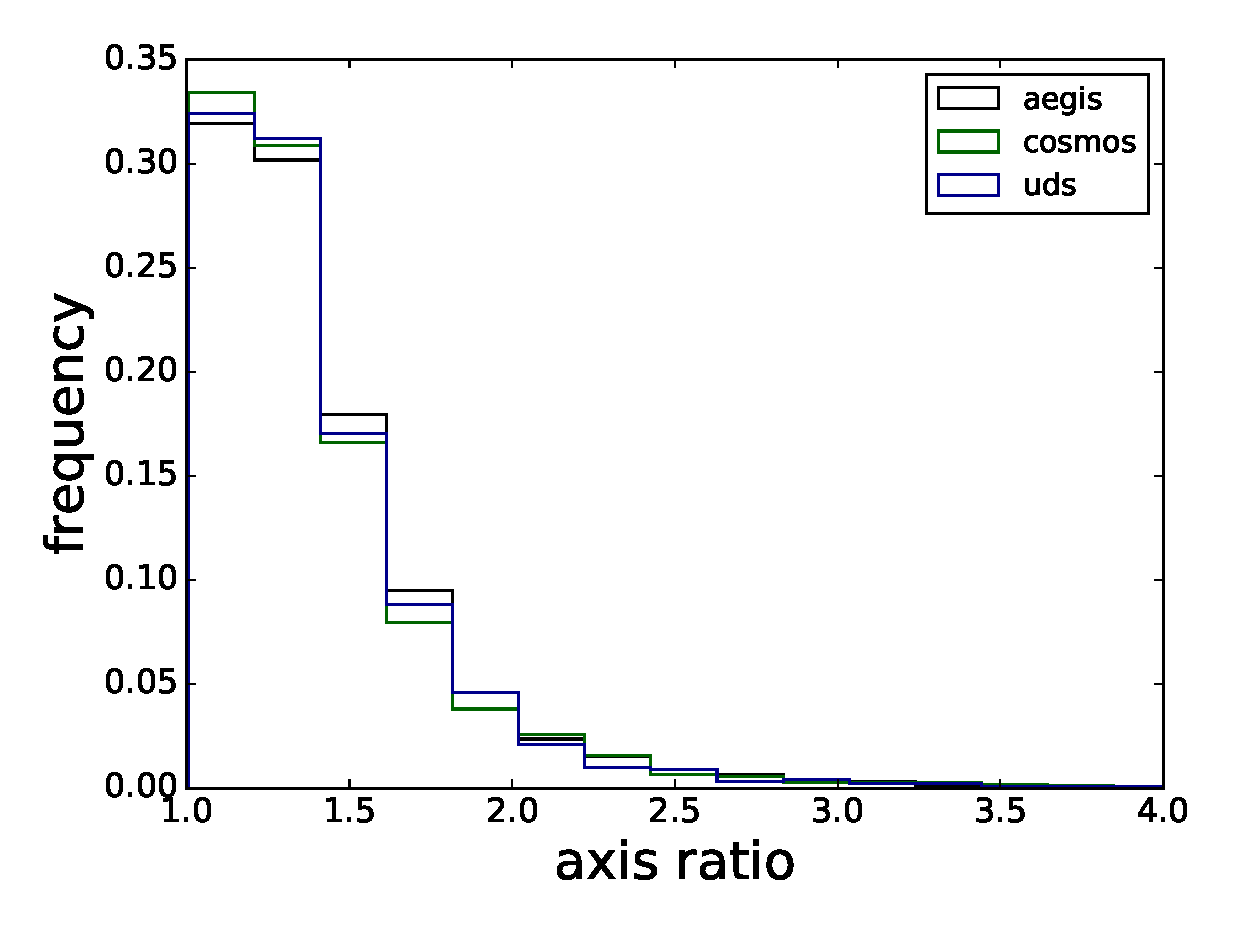
\includegraphics[width=5.0cm]{zhisratio.eps}
    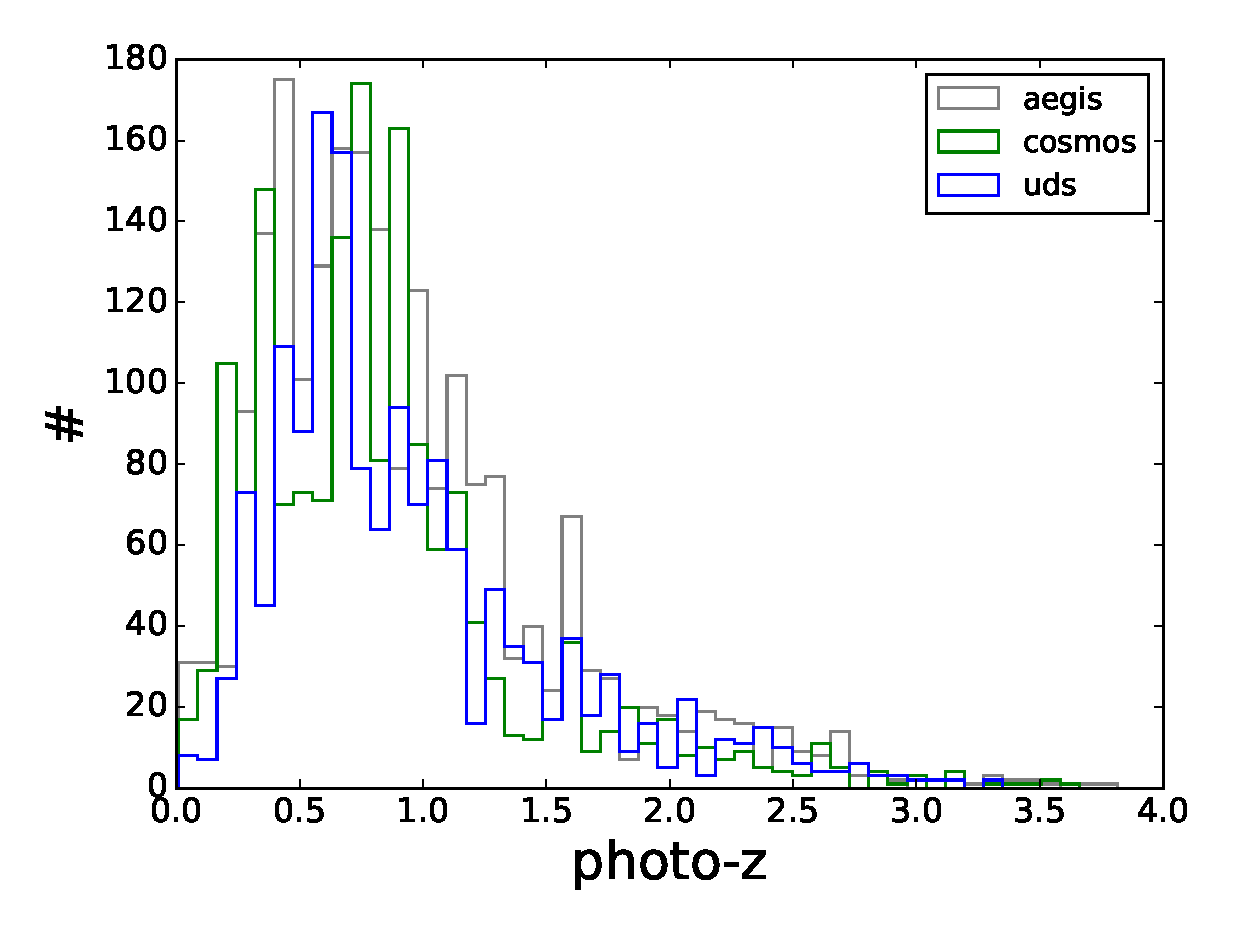
\includegraphics[width=5.0cm]{zhisphotoz.eps}
    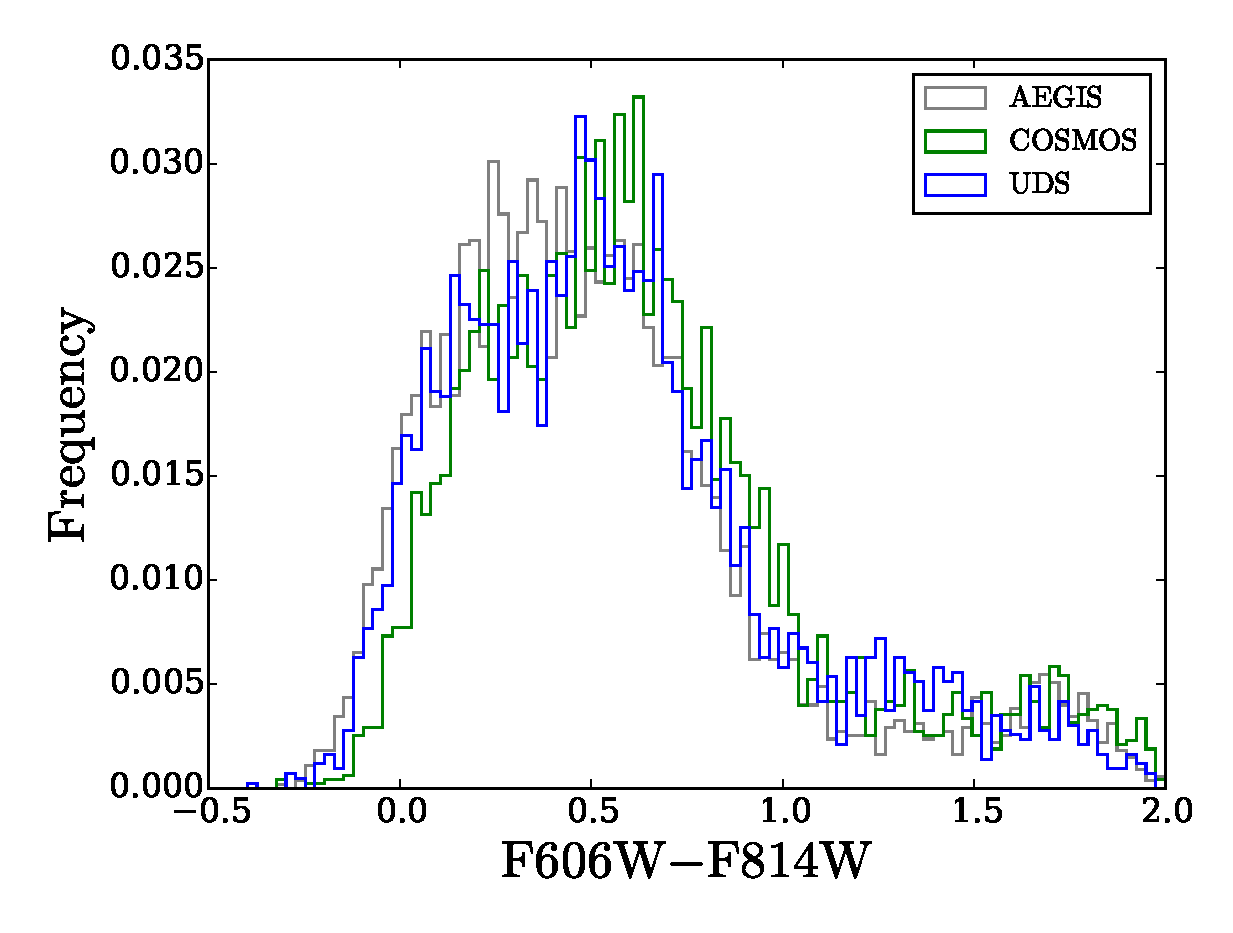
\includegraphics[width=5.0cm]{zhiscolor.eps}}
  \caption{The histogram for basic galaxy properties in our
    sample. The lines with different colours represent galaxies from
    different catalogues (AEGIS, COSMOS, UDS). From left to right: half
    light radius, axis ratio, photometric redshift, and colour
    ($m_{V-I}$).}
  \label{fig:datapro1}
\end{figure*}
%

\subsection{CG bias from CANDELS}
We estimate the CG bias following the same procedure for the simulated galaxy:
\begin{itemize}
  \item
    fit the galaxy using one Sersic component for both band
    images. Some constraints such as Sersic index ($0.5<n<5.0$),
    effective radius ($1<r_e<50$ pixel) and axis ratio ($0.6<q<1.0$)
    are adopted in Galfit.
  \item
    interpolate the SED on each pixel of the galaxy image, and
    generate the galaxy at each wavelength (Eq.\ref{eq:linearitp} -
    \ref{eq:lineareq}), and then integrate over the wavelength to
    simulate the CG and NCG galaxy image.
  \item
    measure the shape of two images and calculate the bias $m$. We
    also apply $6$ different orientation of the images in order
    to reduce the intrinsic shape noise.
\end{itemize}
%
In Fig.\ref{fig:cgbhis}, we show the histogram of the CG bias. The CG
bias in most of the galaxies is smaller than $0.01$ ($94\%$). We did
not perform averaging as we did for the simulated noisy images, which
can further reduce the scatter of the bias. Thus the actual bias,
especially the scatter in the sample, is smaller. In the bottom
panel, we estimate the CG bias using a larger weight function
($2r_h$). As one expected, the bias decreases by about one order of
magnitude.

%
%The red line show the CG bias if we perform lensing instead of shearing
%the images. We can see that the bias becomes larger, and the effect is
%stronger than the PSF variations. However, it is highly possible that we
%overestimate the flexion and the effect due to that, since we did not
%consider the real lens property. In the rest, we only show the result using
%shearing.

%
\begin{figure}
  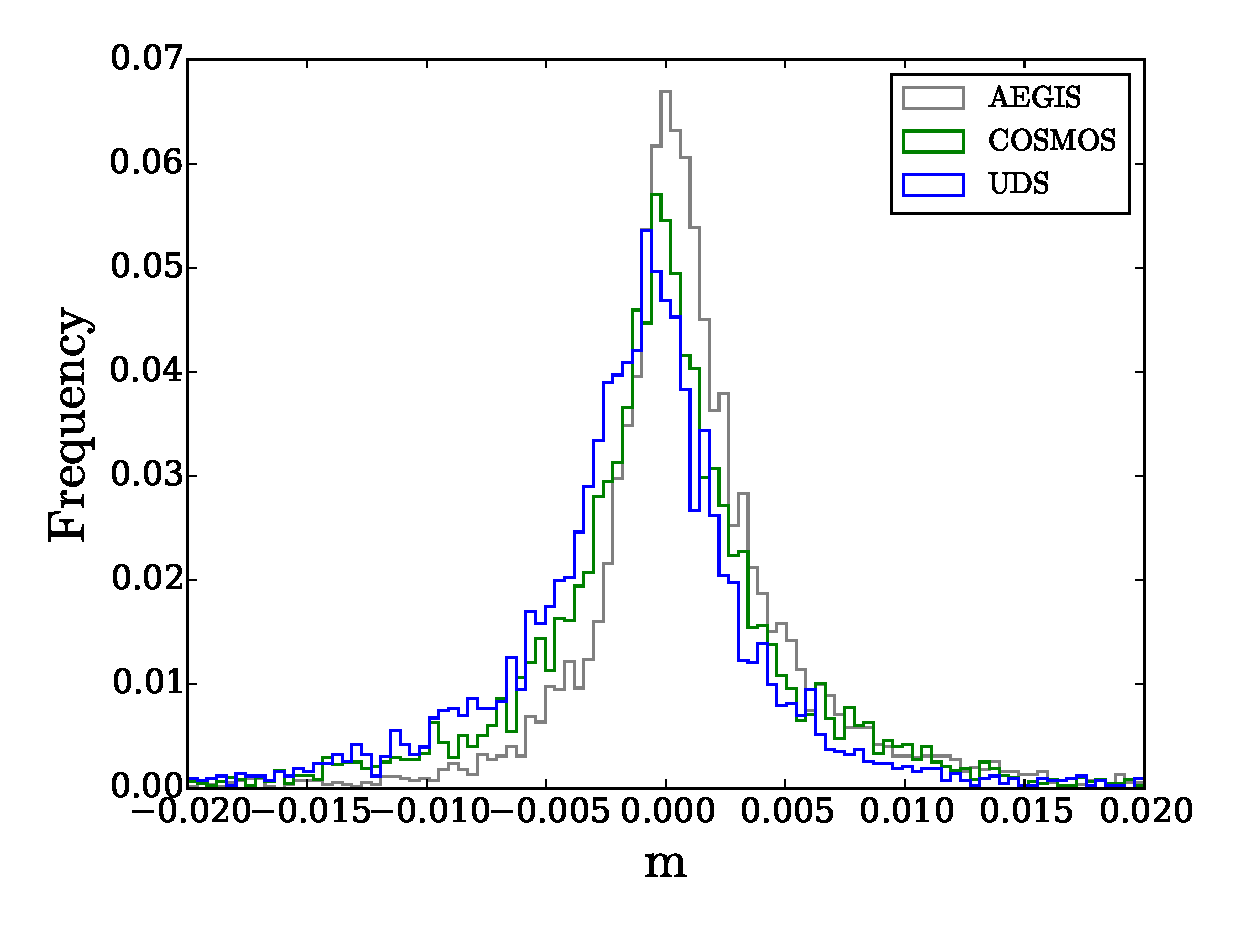
\includegraphics[width=7.0cm]{zhiscgb.eps}
  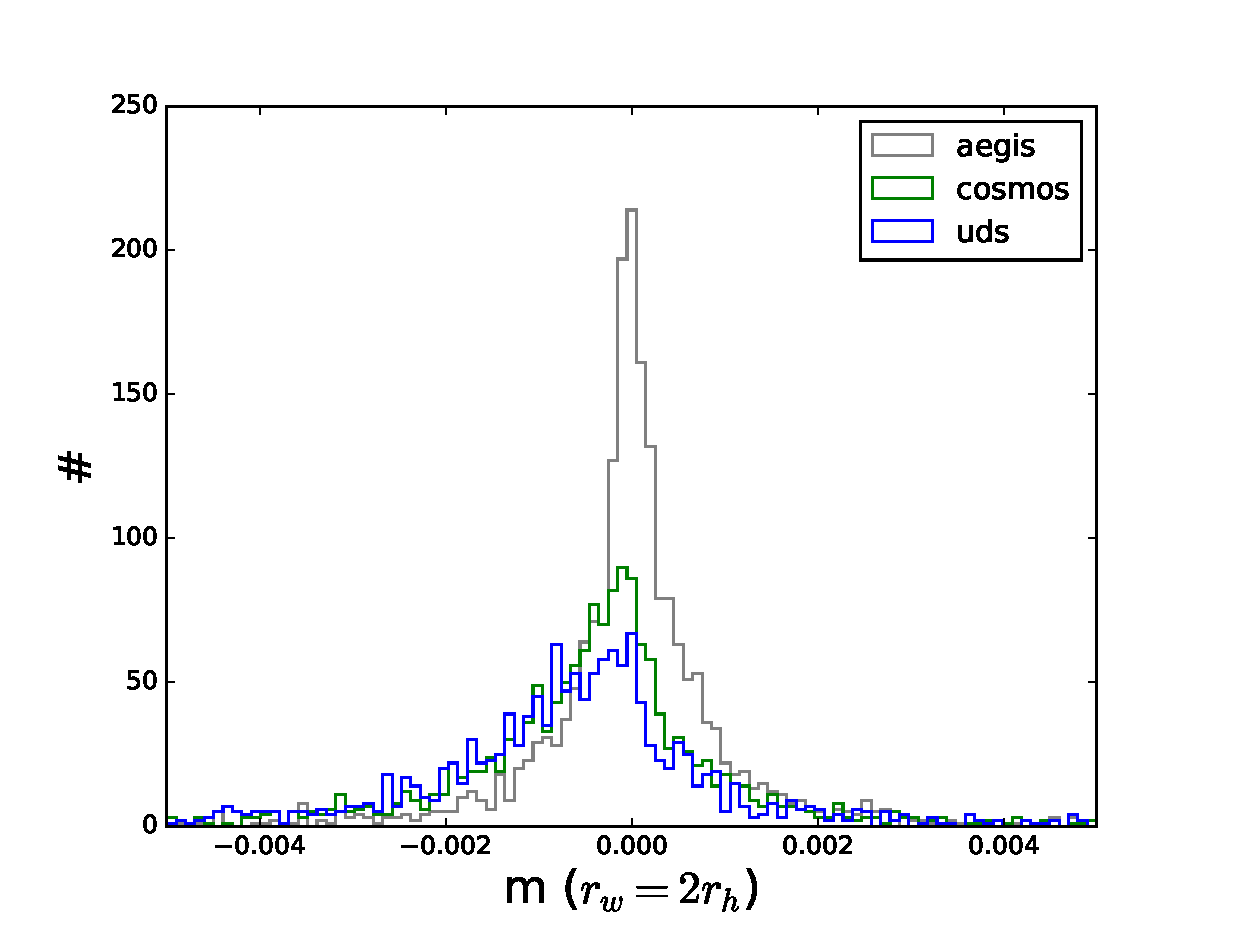
\includegraphics[width=7.0cm]{zhiscgbno.eps}
\caption{CG bias histogram from CANDELS: different colours show the
  result from three catalogues. In the bottom panel we show the CG
  bias using different weight function ($r_w = 2r_h$).  }
\label{fig:cgbhis}
\end{figure}
%
%\begin{figure}
%  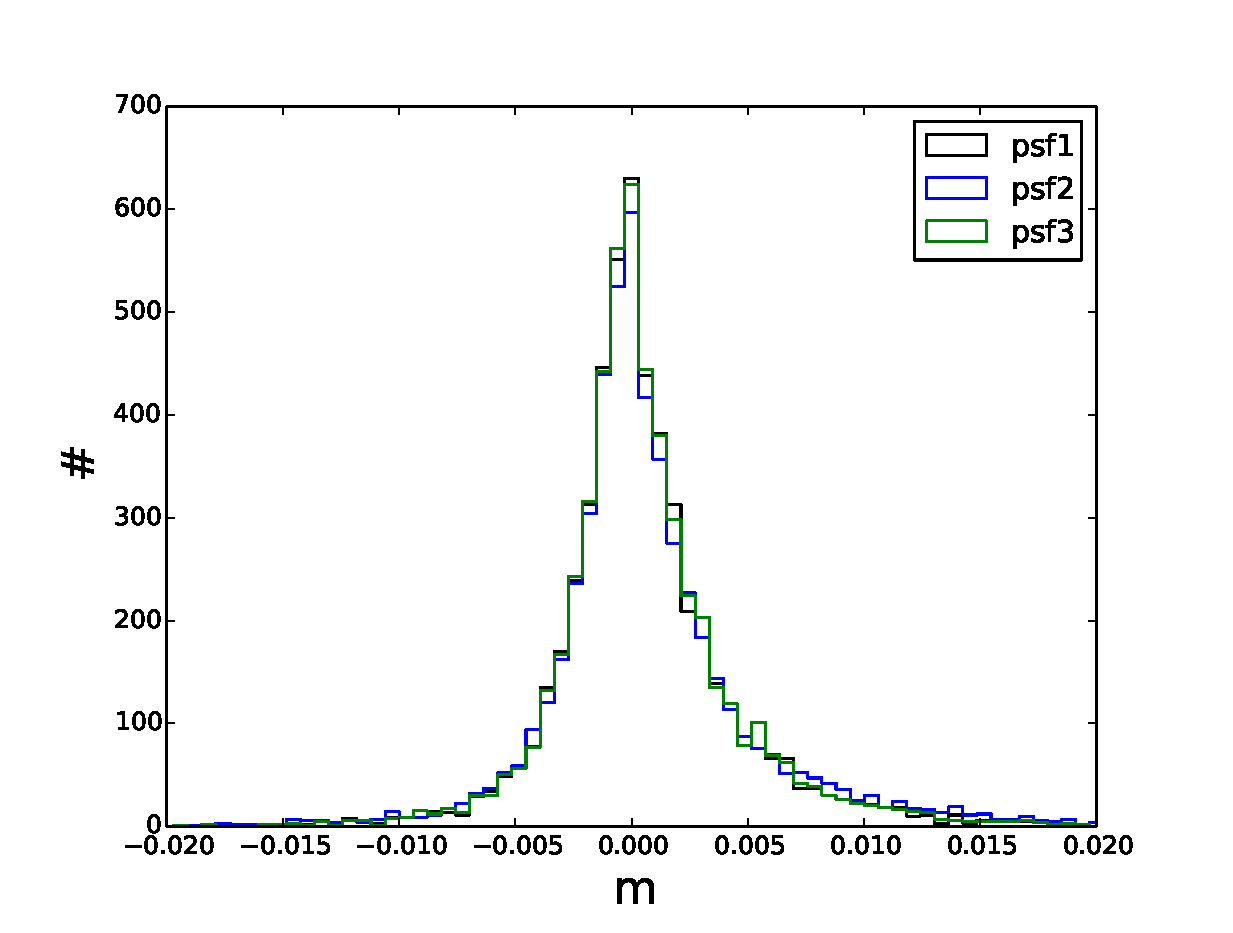
\includegraphics[width=7.0cm]{zcgbhis_psf.eps}
%  \caption{CG bias histogram of CANDELS using three different PSF
%    models from TinyTim.}
%  \label{fig:candelspsf}
%\end{figure}
%
\begin{figure}
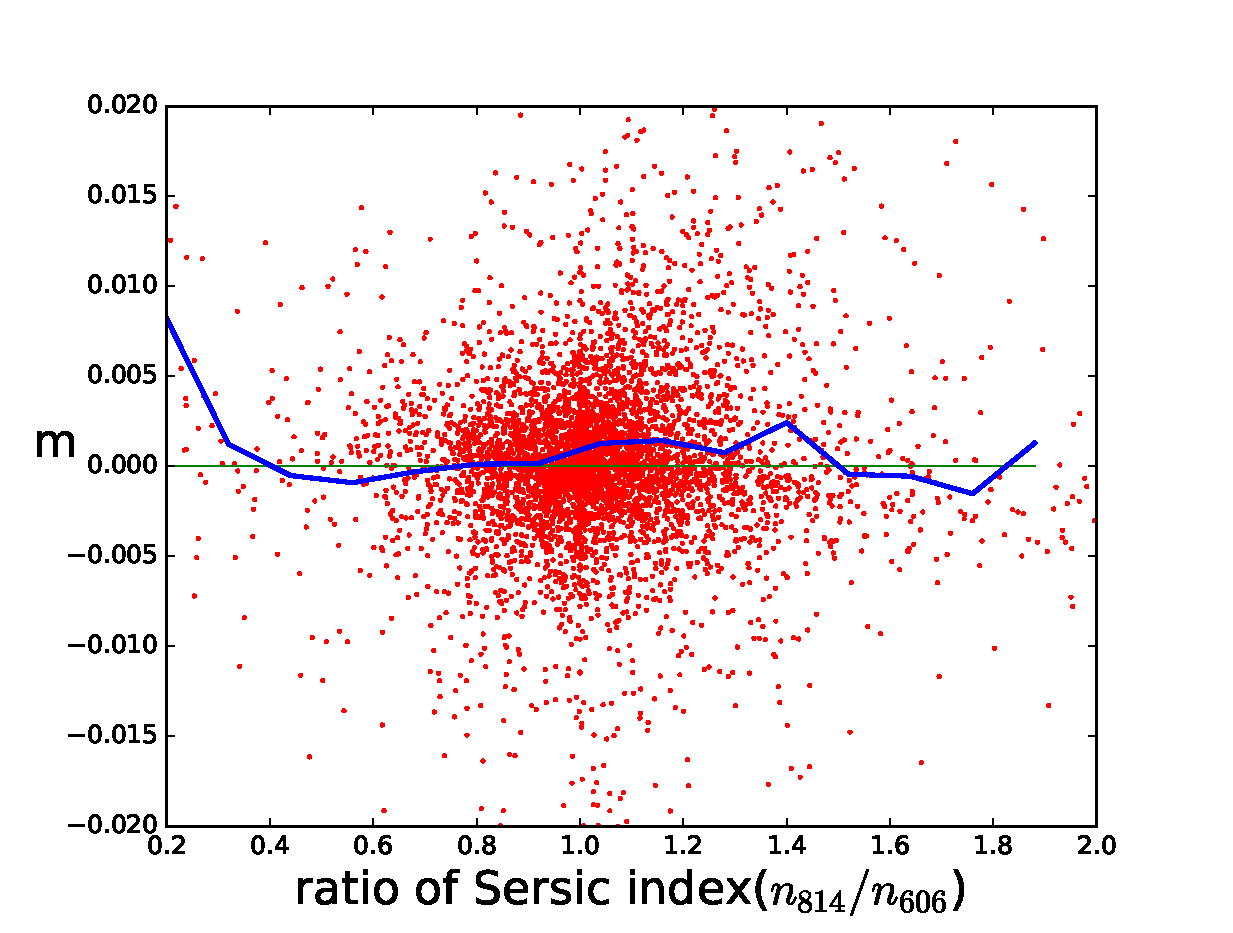
\includegraphics[width=7.0cm]{zcgb-ne17.eps}
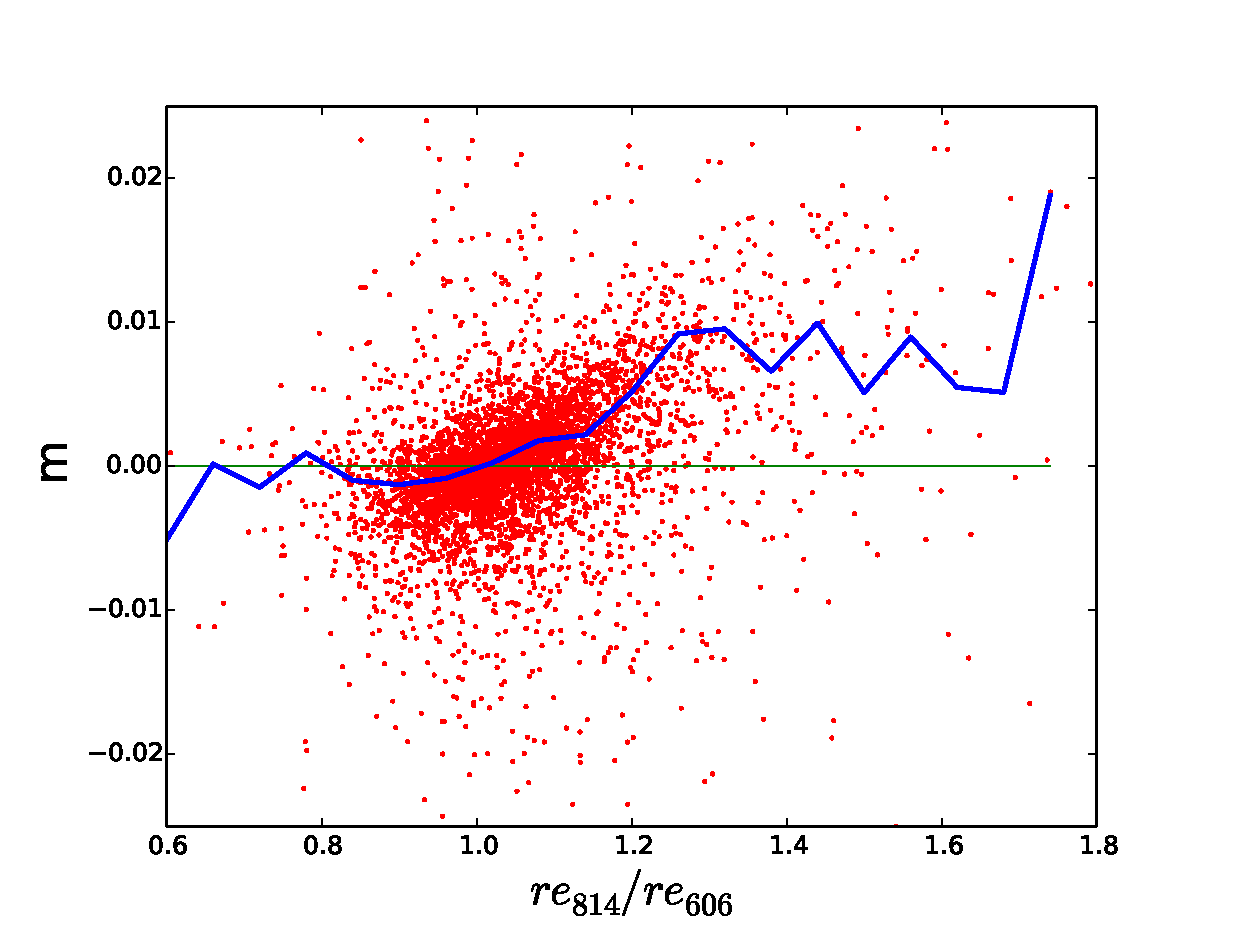
\includegraphics[width=7.0cm]{zcgb-re17.eps}
\caption{CG bias as a function of galaxy properties: ratio of Sersic
  index between two band (top) and effective radius between two bands
  (bottom). The blue lines are the average CG bias over the parameter
  bins.}
\label{fig:cg2fitpar}
\end{figure}
%
\begin{figure}
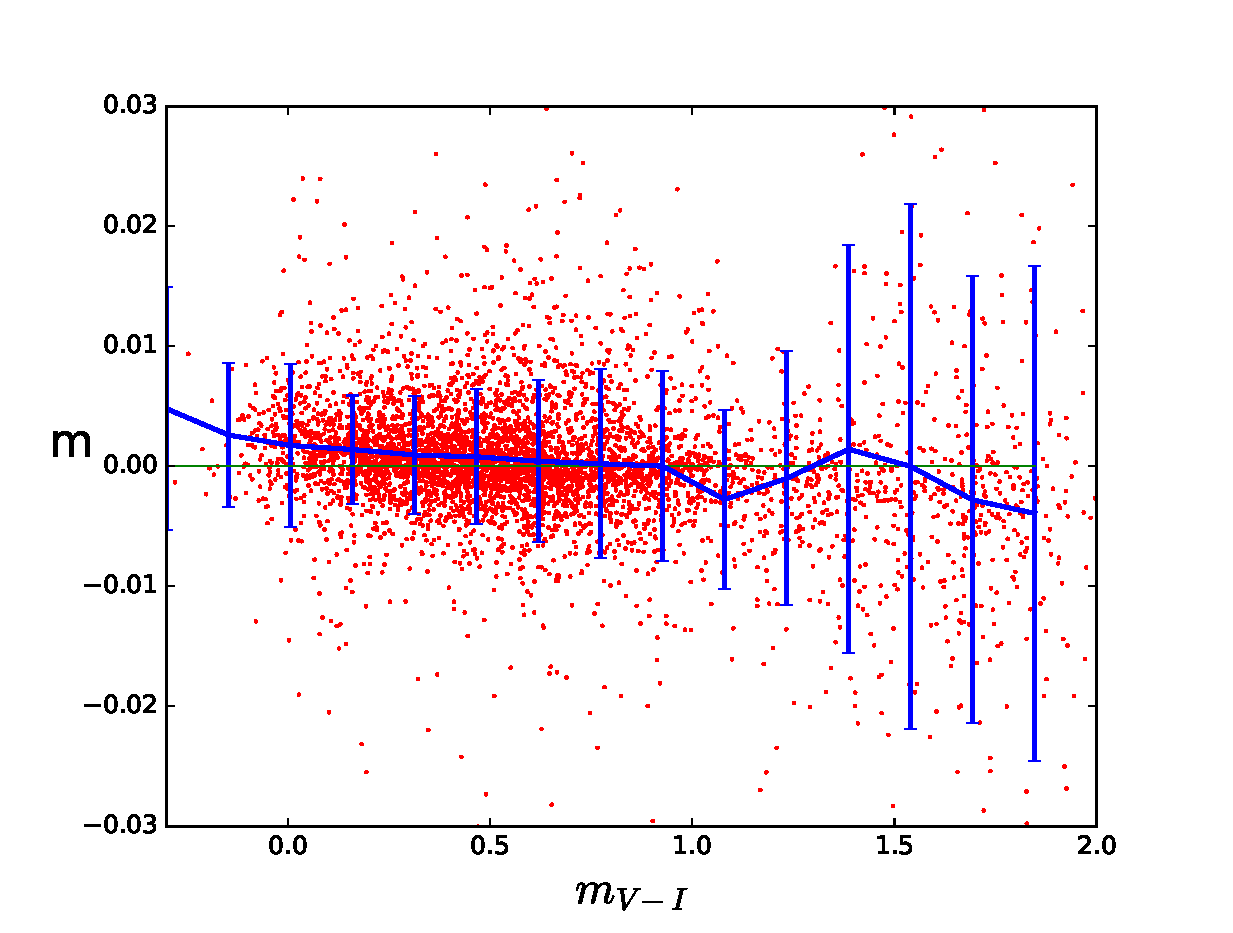
\includegraphics[width=7.0cm]{zcolor17.eps}
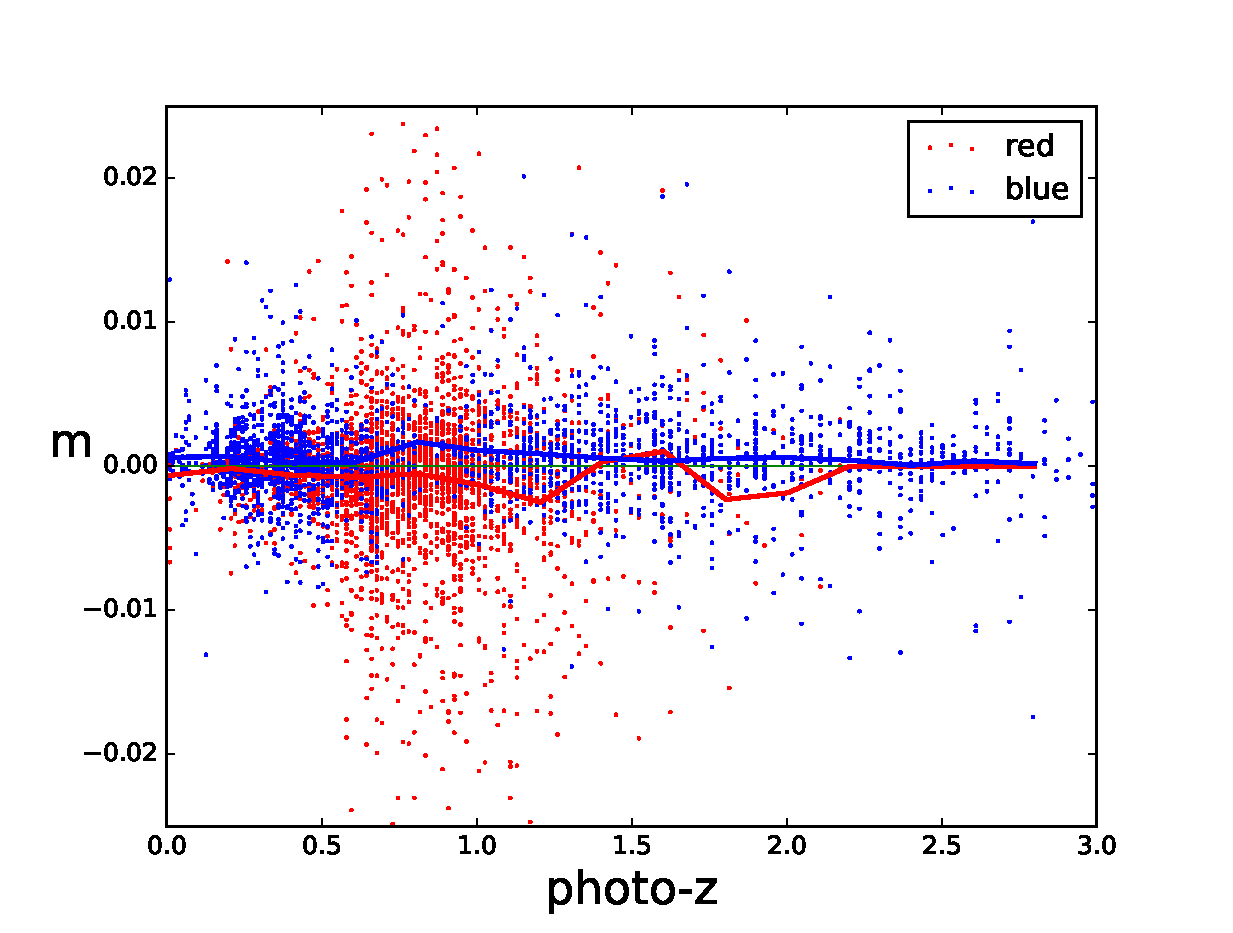
\includegraphics[width=7.0cm]{zphotoz17.eps}
\caption{CG bias as a function of galaxy properties, top: color
  ($m_{V-I}$), bottom: photo-z. In the bottom panel, the red and blue
  points are the bias for red ($m_{V-I}>0.5$) and blue ($m_{V-I}<0.5$)
  galaxies respectively. The lines are the average CG bias in the
  redshift bins.}
\label{fig:cg2color}
\end{figure}
%
\begin{figure}
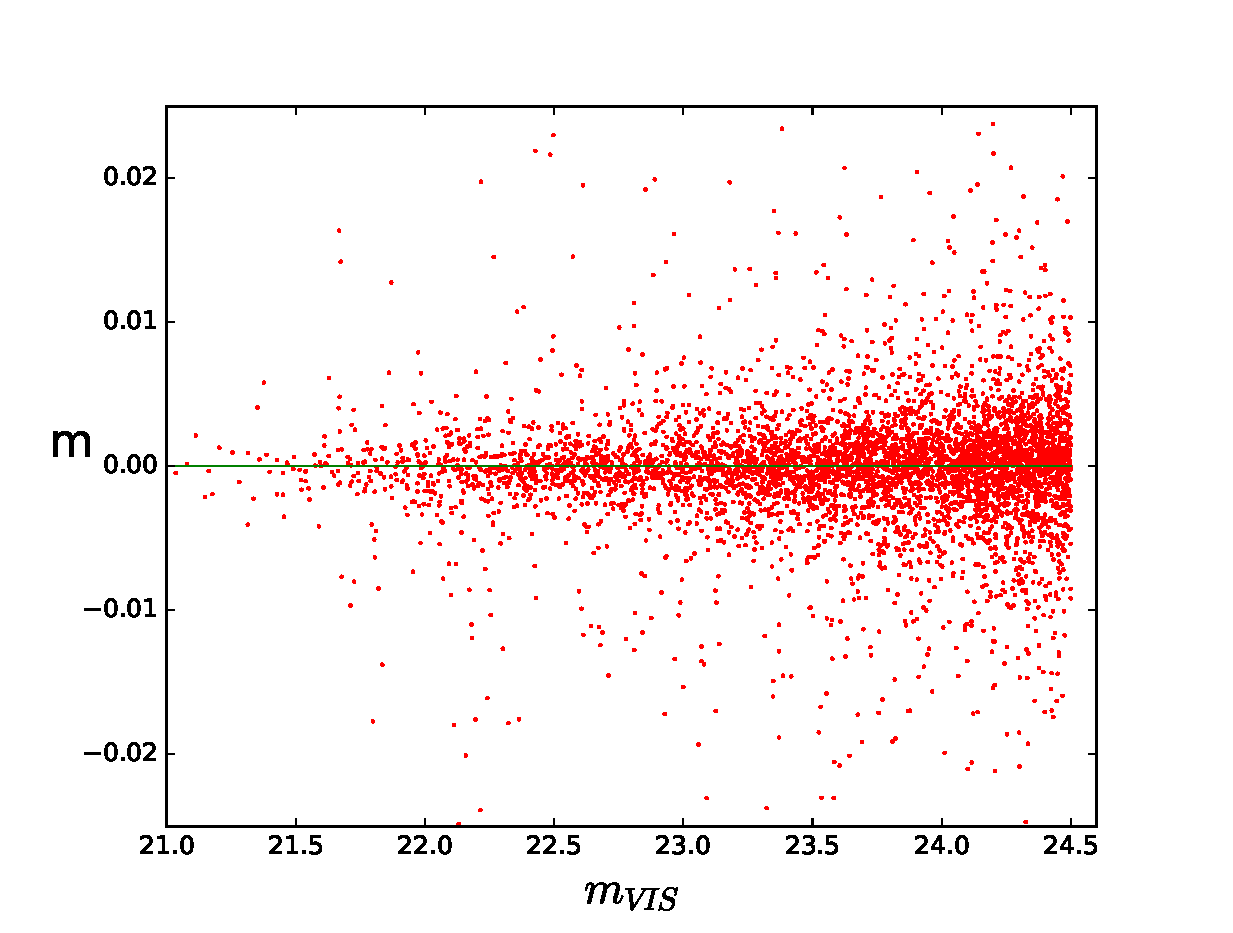
\includegraphics[width=7.0cm]{zcgb-magt17.eps}
\caption{CG bias as a function of mock VIS magnitude. }
\label{fig:cg2magvis}
\end{figure}
%
\begin{figure}
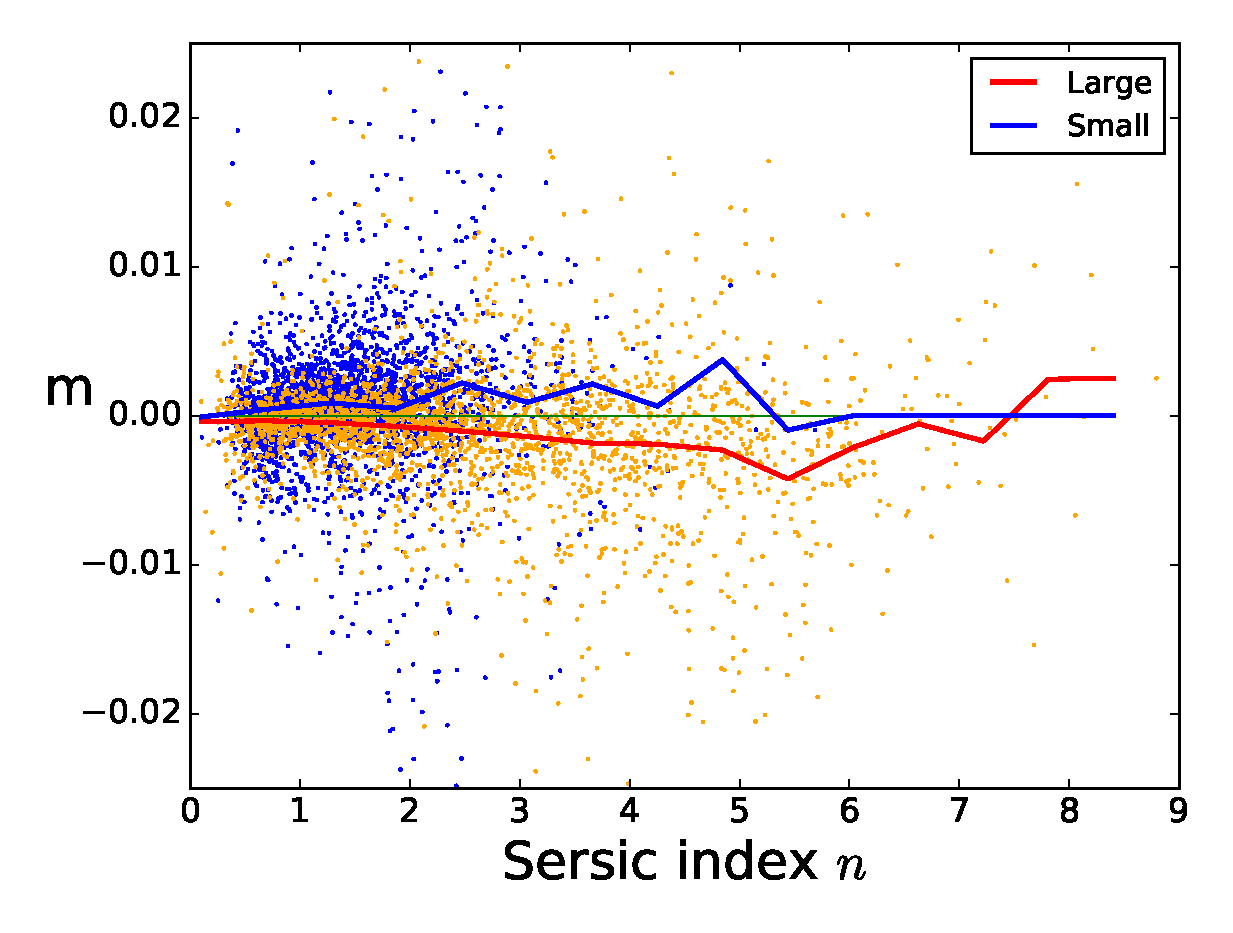
\includegraphics[width=7.0cm]{z2s-ne17.eps}
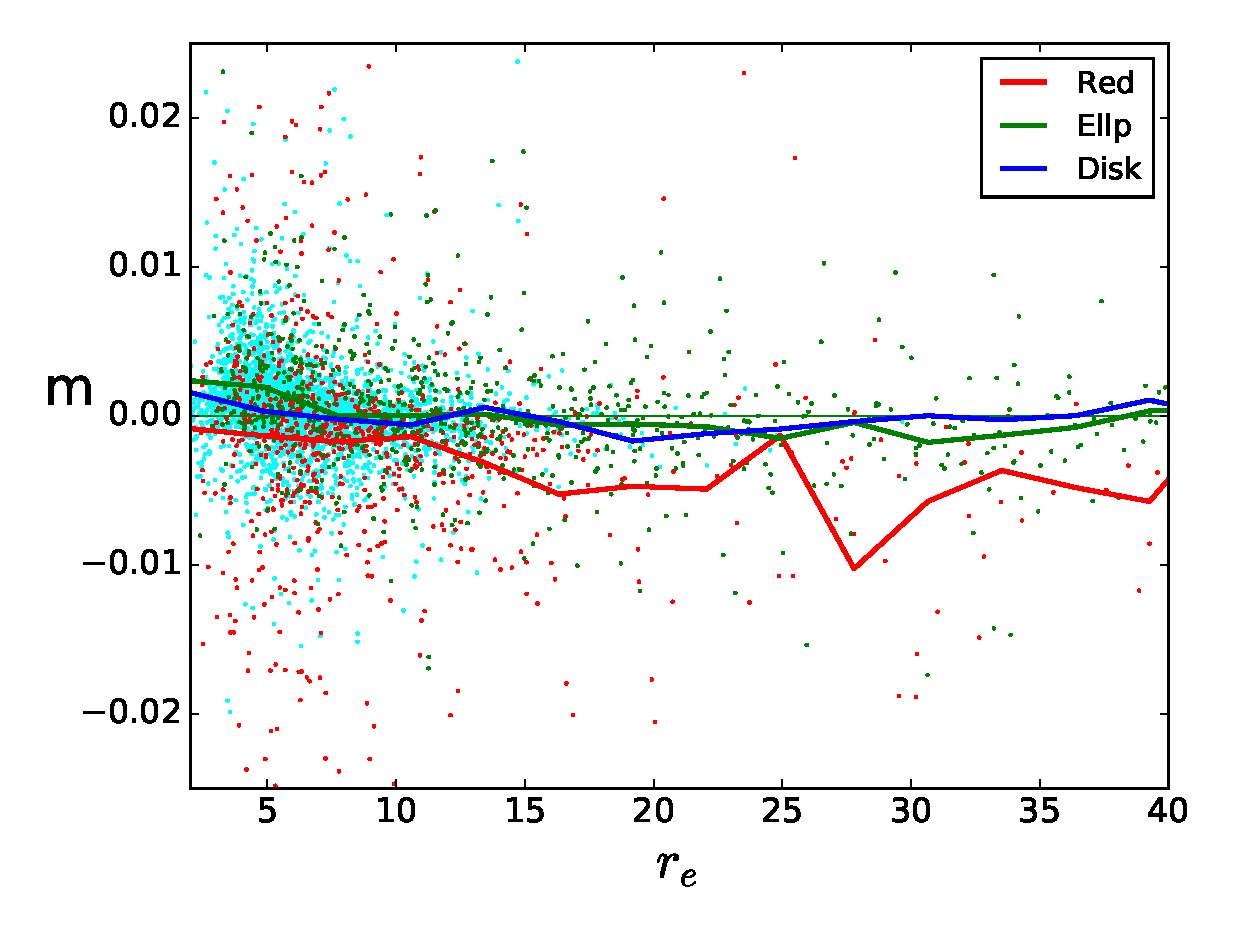
\includegraphics[width=7.0cm]{z2nscl-re17.eps}
\caption{CG bias with Sersic index (top) and effective radius (bottom)
  from the mock VIS images. The unit of radius is a pixel ($=0.05$
  arcsec). In the top panel, the blue (red) is the average of small
  (big) galaxies. In the bottom panel, the red line is average bias of
  red galaxy ($m_{V-I}>1$); the green line is that of elliptical
  galaxy ($n_{Sersic}>2.75$); the blue line is for the disk galaxy.}
\label{fig:cg2re}
\end{figure}
%
The colour gradients as a tracer of galaxy evolution have been found
to be correlate with some aspects. We try to explore relations between
CG bias and the properties of galaxy. First we show the relation
between CG bias with two tracers of the colour gradients: the ratio of
Sersic index from two bands, and the ratio of effective radius from
two bands (Fig. \ref{fig:cg2fitpar}). One can see that there is a
linear relation between the bias and the radius, but for that of
Sersic index it is not obvious. The reason is that the Sersic index is
mainly account for the type of the galaxy, the radius correlates with
the colour gradient directly. Moreover, the CG bias depends on several
factors of the galaxy, e.g. the total size of the galaxy. It is not
surprise to see large bias scatters for the whole sample. In
principle, one expect that when $r_{e606}=r_{e814}$ and
$n_{606}=n_{814}$, the CG bias in principle will be vanish, since the
identical images from two bands will not have a colour gradient. This
is confirmed in our result: the blue line (bin average) in
Fig. \ref{fig:cg2fitpar} meets zero at $r_{e814}/r_{e606}=1$. However,
those colour gradients information will not be available in Euclid. We
also need the relation between the bias with other parameters.


In Fig.\ref{fig:cgbhis}, the galaxies in AEGIS field have more
positive CG bias than the galaxies in the other two. The colour
distribution in AEGIS is different from the other two as well, which
suggests the correlation between the CG bias and the colour of the
galaxy. In Fig.\ref{fig:cg2color}, we show the relation between the CG
bias and the colour of the galaxies. The bias is inversely
proportional to the colour of the galaxies. This is consistent with
the trend of total colour \citep[e.g.][]{2010MNRAS.407..144T}: the
bluer galaxies have positive colour gradients, while the redder ones
have negative gradients. Since this marks a possible transition of two
types of galaxies, we split the galaxy sample into two groups
according to their colour: the red galaxies ($m_{V-I}>0.5$) and the
blue ones ($m_{V-I}<0.5$). They are shown in the bottom panel of
Fig.\ref{fig:cg2color} as a function of redshift. Most of the red
galaxies are located at moderate redshifts, mainly between redshift
$[0.5,1.0]$, while the blue galaxies are either at the lower redshift
($z<0.5$) or higher redshift ($z>1.0$). The CG bias in red galaxies
are obviously more negative than that of the blue ones. It again
confirms that the colour/colour gradients is an important tracer of
the galaxy evolution, since apparently galaxies at different redshift
proceed at different stages of the evolution.

In addition, we stack the images from two bands as our mock VIS band
images, together with the mock VIS magnitude ($m_{VIS}$).  In
Fig.\ref{fig:cg2magvis}, we show the bias as a function of
$m_{VIS}$. There is no obvious dependence on $m_{VIS}$, which seems
conflict with some study of colour gradients,
e.g. \citet{2010MNRAS.407..144T} find tight relation between colour
gradients and $r$-band magnitude. However, there are two points one
needs to notice: 1) the actual $m_{VIS}$ is different from our linear
approximation, also the filter transmission are different of two
telescope. 2) the more important thing is that the wide band magnitude
may not contain sufficient information about the type or colour of
galaxy, thus may not be a good tracer for CG bias.

The VIS image, on the other hand, contains more information
Fig.\ref{fig:cg2re} shows the CG bias with the Sersic index
and the effective radius fitted from the VIS images. In the top panel,
we divide the sample into two groups by the fitted effective radius,
either larger or smaller than $0.35$ arcsec. The small (large)
galaxies are shown by the blue (orange) points, and the blue (red)
line is the bin average.  The large galaxies cover a large range of
Sersic index, have negative average CG bias. Most of small galaxies
have small Sersic index ($<2.5$). The bias of small galaxies are
positive and approximately proportional to the Sersic index. The
scatters of the bias for both large and small galaxies increase with
the Sersic index.
%
In the bottom panel, the galaxies are divide into three groups: the
first is red galaxy whose color is large ($m_{V-I}>1.0$); the second
and third group are the rest galaxies either with large Sersic index
($n>2.25$, elliptical galaxy) or small Sersic index (disk galaxy). The
solid lines show the bin average over effective radius.
%
%\be
%\tilde{m} = a\,r_e+{b\over r_e}+c,
%\elabel{fitcgb}
%\ee
%
%where $r_e$ is the effective radius of the mock VIS image. For disk
%galaxy we have $a=3.8\times10^{-12}$, $b=0.022$, $c=-0.0066$, and for
%elliptical galaxy $a=0.00012$, $b=0.017$ and $c=-0.0069$. The disk
%galaxies have relatively smaller size and smaller CG bias, while the
%elliptical galaxies cover a large range of size and CG bias. Moreover,
%the elliptical galaxies have a stronger dependence on the effective
%radius.
%
We can see that the VIS image alone can also provide an rough
estimation for CG bias, but classification of the galaxies is
necessary. As shown in the figure, the disk galaxies have small bias,
small radius ($<1$ arcsec), and also small bias scatters. The
elliptical galaxies cover large radius range, and the bias is larger
than the disk ones. The bias in red galaxies are significant, and
mainly negative. The scatters of red galaxies are larger than the
other two kinds of galaxies.
%
Extra photometry can definitely provide more constraints on the CG
bias, as it has been shown the correlations between colour gradients and
other properties of galaxy. Moreover, the multi-band
information is required for the photometric redshift study. One can
obtain that for free to calibrate the CG bias. Although the dependence
on the multi-band is different between photometric redshift and CG
bias, the experience from photometric redshift can be used for CG
bias, such as some machine learning algorithms.


We calculate the average bias and the dispersions over the redshift
bins for both red ($m_{V-I}>0.5$) and blue galaxies
(Table\,\ref{table:calibration}). The red galaxies are mainly located
between redshift $(0.4,1.2)$, while the blue galaxies are low density
in redshift $(0.8,1.2)$. The bias from red galaxies are significantly
smaller than that of blue galaxies, as one expected, the colour
gradient in the elliptical galaxies are smaller. The dispersions of
the bias in each bin are large, which probably indicate that in each
bin there are several kinds and sizes of galaxies. Therefore, in
order to calibrate the bias with high precision, one need bigger
galaxy samples. From our simulation, we need about $200$ galaxies for
one type of galaxy in every redshift bin. If we make rough bins, for
instance, 2 types of colour: red and blue; 5 different sizes from
about $0.1$ arcsec to $1.0$ arcsec (Fig.\ref{fig:cg2re}), and 5
redshift bins, at least $20 000$ galaxies are required.  For more
realistic SED classifications and redshift bins, several times larger
sample are also necessary.


\begin{center}
\begin{table}
  \begin{tabular}{llll}
    \hline
    photo-z    &$Number$  &$\bar{m}$  &$\sigma_m$ \\
    \hline
    $0-0.4$   &187  &$-1.3\times10^{-3}$  &$0.012$\\
    $0.4-0.8$  &1415 &$-7.6\times10^{-4}$  &$0.011$\\
    $0.8-1.2$  &1116 &$-1.0\times10^{-3}$  &0.017\\
    $>1.2$  &245  &$-2.1\times10^{-3}$  &0.015\\
    \\
    $0-0.4$  &667  &$6.6\times10^{-4}$  &0.0026\\
    $0.4-0.8$ &513  &$2.8\times10^{-4}$  &0.0028\\
    $0.8-1.2$ &187  &$1.2\times10^{-3}$  &0.0041\\
    $>1.2$  &935  &$5.4\times10^{-4}$  &0.0046\\
    \hline
  \end{tabular}
  \caption{\label{table:calibration}The number, average CG bias and dispersion
  in redshift bins for blue (bottom half) and red (top half) galaxies. }
\end{table}
\end{center}

%\be
%c=m{e_{\rm PSF} \over P_{\gamma}P_{ePSF}},
%\ee
%follow Massey $P_{ePSF}=1$, $P_{\gamma}=0.93$ and using a conservative choice, which corresponds to the maximum value for the polarization allowed for the Euclid PSF $e_{PSF}=0.07$.


\section{Summary and Discussion}
In the image survey for weak gravitational lensing, the wide band
filter can provide high signal-to-noise images and large coverage of
redshift range. There is however a shape bias due to the chromatic
shape of galaxy and the PSF, which is named as colour gradient
bias. For very wide band surveys, such as Euclid, this effect can
cause a non-negligible bias.
%
In this work, we exam such a kind of bias in measuring the shape of a
galaxy using both simulated images and real data taken from the HST
ACS CANDELS survey. In the simulated galaxy images, we confirm the
bias behaviour from previous results (\citetalias{Semboloni13}). We further apply the
calibration method to the noisy images in the simulations, and find
that with reasonable signal-to-noise ratio (SNR$=15$) and sufficient
numbers of galaxies ($300$ images for one type of galaxy in one
redshift bin), we can estimate the CG bias to a high precision.
However, the underestimate cannot be avoided due to strong emission
lines, or the uneven SED of source galaxies. Moreover, the simulations
are performed with only two galaxy models, and the SNR of the
simulated images in two bands are assigned with equal value. In
reality, the relation between the SNR with the size and SED of the
galaxies has to be taken into account.
%
We also perform comparison of TinyTim and star PSF models. The
inaccuracy, especially that due to the binary stars, will cause errors
in estimating the CG bias.


In the estimation using CANDELS data, we select the images from two
filters (F606W, F814W). For most of the galaxy, the bias ($|m|$) is
smaller than $0.01$.  As we find from simulated images, the estimation
using noisy image has a large scatter, thus the CG bias in reality may
be even smaller than that shown here.
%
In our sample of galaxies, the CG bias shows a correlation with the
colour of galaxies, and a linear relation with the ratio of two band
images. We also generate the mock VIS band images. From the parameters
of the image (Sersic index and effective radius), one can classify the
galaxy in order to obtain tighter constraints on the bias. For example,
the galaxies with small Sersic index, i.e. disk-like, have smaller CG
bias. On the other hand, those with large Sersic index have large bias
and also bias variation. The relations show consistent results about
the colour gradient dependence on the properties of galaxy
\citep[e.g.][]{2010MNRAS.407..144T}. However, since the CG bias also
depends on the relative size with respect to the PSF, the dependence
of CG bias is certainly more complicate. We did not provide any
fitting formula for the bias at current sample, since the scatters are
too large. More importantly, it has to be performed according to the
types or morphology of the galaxies, which require larger sample of data.

The multi-band photometry from several bands, which can be used to
estimate the redshift, can be also use for the CG bias analysis.
Although the redshift dependence is not significant in our sample of
galaxies, this may not be the case for a larger survey, or if we look
at the bias according to the type of galaxy. Moreover, the colour of
galaxy also indicates the evolution history, or the large scale tide
force.  It can be also used for the study of intrinsic alignment
analysis in weak lensing \citep[e.g.][]{2015SSRv..193....1J}.
Therefore, the dependence of the CG bias on the colour of the galaxies
will further increase the sysmatics of the intrinsic alignment. The
detail behaviour will require large cosmological simulations, which is
beyond the scope of this paper, but definitely needs further studies for
the project such as Euclid.

The role of environment on the colour gradients is not clear. On the
one hand, it has been shown that colour gradients depend on the
environment where galaxies reside, with steeper colour gradients in
poor rather than rich clusters \citep[e.g.][]{2005ApJ...626L..19L},
which is possible due to the different processes during galaxy
formation. On the other hand, in recent study using integral field
spectra from SDSS-IV, the metallicity gradients show weak or no
correlation with density environment \citep{2017MNRAS.465.4572Z}. In
any cases, close galaxy pairs or nearby bright star(s) may also cause
weak brightness/colour gradient, which will affect our estimate for CG
bias as well. Moreover, in the calibration we linearly interpolate the
SED on pixels from two bands. Some advanced method to estimate the SED
\citep[e.g.][]{2016A&A...589A...2J} may help to improve the
calibration of the bias.

In this work, we use the brightness moments to estimate the
ellipticity of the galaxy. The PSF correction is not taken into
account. The bias thus will appear in every method of measurement.
However, the bias using the measurement method for real data
will be different, since every method has its own property and weight
function. The CG bias will have method-dependent properties as well,
although they will in principle have same dependence on the colour
gradient of the galaxy images. As the first step of the CG bias
analysis, we did not adopt any specific method in order to obtain
general properties of the CG bias. Before the real analysis of Euclid
data, one needs to study the bias with specific methods and simulated
images with real properties in the Euclid weak lensing survey.

%
%Moreover, as we point out that higher order image distortions, such as
%flexion may increase the CG bias. It can be seen from our analysis
%using both simulated and CANDELS data. Although the higher order
%effect can be neglected most times, it can still significantly
%increase the CG bias when the source images are located close to the
%strong lensing region. Therefore, such a kind of effect may cause
%significant bias in the strong lensing analysis using wide band
%images. In galaxy-galaxy lensing and cluster lensing, one needs to
%be careful about such higher order effects as well.

\section*{Acknowledgments}

We would like to thank Emiliano Merlin, Marco Castellano for helping
on SExctractor and Galfit, Gary Berstein, Adam Rogers and
also in general, the members of the Euclid Consortium for useful
discussions.  XE and VFC are funded by Italian Space Agency (ASI)
through contract Euclid -IC (I/031/10/0) and acknowledge financial
contribution from the agreement ASI/INAF/I/023/12/0. XE is also partly
support by NSFC Grant No. 11473032. JR is supported by JPL, which is
run by Caltech under a contract for NASA, and is supported by grant
NASA ROSES 12-EUCLID12- 0004. The fast Fourier transforms are supplied
by the FFTW library \citep{fftw05}. We use CFITSIO
\citep{1999ASPC..172..487P} for the FITS file.

\bibliographystyle{aa}
\bibliography{cbias}

\end{document}
